\documentclass[12pt,a4paper]{article}

% Core packages
\usepackage[utf8]{inputenc}
\usepackage[T1]{fontenc}
\usepackage[english]{babel}
\usepackage[margin=2.2cm]{geometry}
\usepackage{microtype}
\usepackage{hyphenat}

% Enhanced formatting packages
\usepackage{fancyhdr}
\usepackage{titlesec}
\usepackage{titling}
\usepackage{enumitem}
\usepackage{parskip}
\usepackage{setspace}

% Math and technical packages
\usepackage{amsmath}
\usepackage{amsfonts}
\usepackage{amssymb}
\usepackage{mathtools}

% Graphics and visualization
\usepackage{graphicx}
\usepackage{float}
\usepackage{subfig}
\usepackage{caption}
\usepackage{subcaption}

% Tables
\usepackage{booktabs}
\usepackage{array}
\usepackage{tabularx}
\usepackage{multirow}
\usepackage{longtable}

% --- in your preamble ---
\usepackage{tikz}
\usetikzlibrary{positioning,shapes.geometric,shapes.symbols,arrows.meta,calc}


% TikZ for diagrams
\usepackage{tikz}
\usepackage{pgfplots}
\pgfplotsset{compat=1.18}
\usetikzlibrary{
    positioning,
    shapes.geometric,
    arrows.meta,
    calc,
    decorations.pathreplacing,
    patterns,
    backgrounds
}

% Code and algorithms
\usepackage{listings}
\usepackage{algorithm}
\usepackage{algpseudocode}

% Colors and hyperlinks
\usepackage{xcolor}
\usepackage{hyperref}
\usepackage{url}
\usepackage{tcolorbox}

% CIAF Color Scheme
\definecolor{ciafblue}{RGB}{41, 128, 185}
\definecolor{ciafgray}{RGB}{127, 140, 141}
\definecolor{ciafdarkblue}{RGB}{22, 67, 91}
\definecolor{ciaflightblue}{RGB}{174, 214, 241}
\definecolor{ciafgreen}{RGB}{39, 174, 96}
\definecolor{ciaforange}{RGB}{230, 126, 34}
\definecolor{ciafred}{RGB}{231, 76, 60}
\definecolor{ciaflight}{RGB}{240,245,250}
\definecolor{success}{RGB}{40,167,69}
\definecolor{warning}{RGB}{255,193,7}
\definecolor{danger}{RGB}{220,53,69}

% Custom boxes
\newtcolorbox{executivebox}{
    colback=ciaflight,
    colframe=ciafblue,
    boxrule=1pt,
    arc=5pt,
    left=10pt,
    right=10pt,
    top=10pt,
    bottom=10pt
}

\newtcolorbox{valuebox}{
    colback=success!10,
    colframe=success,
    boxrule=1pt,
    arc=3pt,
    left=8pt,
    right=8pt,
    top=8pt,
    bottom=8pt
}

\newtcolorbox{technicalbox}{
    colback=ciaflight,
    colframe=ciafdarkblue,
    boxrule=1pt,
    arc=3pt,
    left=8pt,
    right=8pt,
    top=8pt,
    bottom=8pt
}

\newtcolorbox{infobox}{
    colback=blue!5,
    colframe=blue!75!black,
    boxrule=0.5pt,
    arc=2pt,
    left=6pt,
    right=6pt,
    top=6pt,
    bottom=6pt
}

% Code listing setup with enhanced line breaking
\lstset{
    language=Python,
    basicstyle=\ttfamily\footnotesize,
    keywordstyle=\color{ciafblue}\bfseries,
    commentstyle=\color{ciafgray}\itshape,
    stringstyle=\color{ciaforange},
    numberstyle=\tiny\color{ciafgray},
    backgroundcolor=\color{gray!5},
    frame=single,
    frameround=tttt,
    framerule=0.5pt,
    rulecolor=\color{ciafgray!50},
    breaklines=true,
    breakatwhitespace=true,
    postbreak=\mbox{\textcolor{red}{$\hookrightarrow$}\space},
    breakindent=1.5em,
    prebreak=\raisebox{0ex}[0ex][0ex]{\ensuremath{\hookleftarrow}},
    tabsize=4,
    showstringspaces=false,
    numbers=left,
    numbersep=8pt,
    xleftmargin=15pt,
    xrightmargin=5pt,
    captionpos=b,
    columns=flexible,
    keepspaces=true,
    mathescape=false,
    extendedchars=true
}

% Configure hyperref
\hypersetup{
    colorlinks=true,
    linkcolor=ciafblue,
    filecolor=ciaforange,
    urlcolor=ciafblue,
    citecolor=ciafblue,
    pdftitle={CIAF + LCM: Cryptographic Audit Framework for Verifiable AI Governance},
    pdfauthor={Denzil James Greenwood},
    pdfsubject={Research Disclosure \& Technical Portfolio 2025},
    pdfkeywords={AI Governance, Cryptographic Verification, Audit Trails, EU AI Act, NIST AI RMF}
}

% Line breaking improvements
\tolerance=1000
\emergencystretch=3em
\hyphenpenalty=10000
\exhyphenpenalty=100

% Page layout
\geometry{
    a4paper,
    left=2.5cm,
    right=2.5cm,
    top=3cm,
    bottom=3cm,
    headheight=14.5pt
}

% Header and footer
\pagestyle{fancy}
\fancyhf{}
\fancyhead[L]{\textcolor{ciafgray}{\small CIAF + LCM Research Portfolio}}
\fancyhead[R]{\textcolor{ciafgray}{\small \thepage}}
\fancyfoot[C]{\textcolor{ciafgray}{\small Cognitive Insight Audit Framework • Research Disclosure 2025}}
\renewcommand{\headrulewidth}{0.4pt}
\renewcommand{\footrulewidth}{0.4pt}
\renewcommand{\headrule}{\hbox to\headwidth{\color{ciafgray}\leaders\hrule height \headrulewidth\hfill}}
\renewcommand{\footrule}{\hbox to\headwidth{\color{ciafgray}\leaders\hrule height \footrulewidth\hfill}}

% Title formatting
\titleformat{\section}
  {\Large\bfseries\color{ciafdarkblue}}
  {\thesection}{1em}{}

\titleformat{\subsection}
  {\large\bfseries\color{ciafblue}}
  {\thesubsection}{1em}{}

\titleformat{\subsubsection}
  {\normalsize\bfseries\color{ciafblue}}
  {\thesubsubsection}{1em}{}

\begin{document}

% Title page
\begin{titlepage}
\centering
\vspace*{1cm}

{\Huge\bfseries\color{ciafdarkblue} CIAF + LCM: Cryptographic Audit Framework for Verifiable AI Governance\par}
\vspace{0.5cm}
{\LARGE\color{ciafblue} Research Disclosure \& Technical Portfolio 2025\par}
\vspace{2cm}

{\Large\textbf{Author:} Denzil James Greenwood\par}
\vspace{0.5cm}
{\large\textbf{Affiliation:} Independent Researcher\par}
\vspace{0.5cm}
{\large\textbf{Contact:} https://CognitiveInsight.ai or founder@cognitiveinsight.ai \par}
\vspace{0.5cm}
{\large\textbf{Date:} October 28, 2025\par}
\vspace{0.5cm}
{\large\textbf{Version:} 1.0.0\par}

\vspace{2cm}

\begin{executivebox}
\textbf{Research Contribution Statement}

This portfolio presents the Cognitive Insight Audit Framework (CIAF) and Lazy Capsule Materialization (LCM™) as a complete research contribution for cryptographically verifiable AI governance. The work addresses critical gaps in AI audit trail management, regulatory compliance automation, and cross-industry deployment patterns.

\vspace{0.5cm}

\textbf{Independent Research Declaration} 

This work represents independent academic research conducted outside of any institutional or commercial affiliation. The author seeks institutional collaboration, peer review, and funded research partnerships while maintaining academic integrity and open access principles. While the research itself is conducted independently without commercial bias, the Apache 2.0 license explicitly permits commercial use and modification of the software components to encourage broad adoption and community development.
\end{executivebox}

\vfill

\begin{center}
\textcolor{ciafgray}{\rule{0.8\textwidth}{0.4pt}}\\
\vspace{0.5cm}
\textbf{\large Integrated Research Documentation}\\
\vspace{0.3cm}
\textit{Conceptual Theory → Formal Data Model → Implementation Standard}\\
\vspace{0.5cm}
\textcolor{ciafgray}{\rule{0.8\textwidth}{0.4pt}}
\end{center}

\vfill
\end{titlepage}

% Table of Contents
\tableofcontents
\newpage

% 1. Executive Overview
\section{Executive Overview}

\begin{executivebox}
\textbf{Cognitive Insight™ Mission:} Enabling verifiable AI governance through cryptographically secured, evidence-based audit trails that ensure compliance with emerging regulatory frameworks including the EU AI Act and NIST AI Risk Management Framework.
\end{executivebox}

\subsection{Framework Summary}

The Cognitive Insight Audit Framework (CIAF) with Lazy Capsule Materialization (LCM™) represents a paradigm shift in AI governance technology. Rather than retrofitting existing systems with compliance overlays, CIAF implements cryptographically verifiable audit trails from the ground up, ensuring that every decision, training event, and inference operation can be independently verified and reconstructed.

\textbf{Core Innovation:} CIAF + LCM delivers \textbf{cryptographically verifiable, deferred-evidence audit trails} for AI systems ensuring compliance with the EU AI Act and NIST AI RMF through:

\begin{itemize}
\item \textbf{Approximately 85\% storage reduction} through lazy materialization protocols
\item \textbf{Automated compliance mapping} across 20+ industry verticals
\item \textbf{Cross-platform verification} via canonical JSON serialization (RFC 8785)
\item \textbf{Real-time regulatory alignment} with evolving AI governance requirements
\end{itemize}

\begin{infobox}
\textbf{Quick Start: CIAF CLI Demo}
\begin{enumerate}
\item \textbf{Generate:} \texttt{ciaf generate --model model.pkl --data input.json}
\item \textbf{Batch:} \texttt{ciaf batch --receipts ./receipts/ --output proof.merkle}
\item \textbf{Verify:} \texttt{ciaf verify --proof proof.merkle --receipt receipt\_id}
\item \textbf{Materialize:} \texttt{ciaf materialize --receipt receipt\_id --evidence evidence.json}
\end{enumerate}
\end{infobox}

\textbf{Deployment Posture.} CIAF+LCM is designed to run co-located with model training/inference (SDK/CLI) so that evidence capture, commitments, WORM sealing, and verification occur inside your controlled environment (on-prem, VPC, or air-gapped). An HTTP API may be exposed internally if desired, but it is not required for the core audit-trail guarantees (deferred materialization, Merkle batch proofs, cryptographic verification).

\subsection{Research Context \& Objectives}

As an \textbf{independent researcher}, this work seeks:

\begin{valuebox}
\begin{itemize}
\item \textbf{Institutional Collaboration:} Partnership with AI governance labs, regulatory sandboxes, and academic research centers
\item \textbf{Peer Review \& Validation:} Academic publication and conference presentation opportunities
\item \textbf{Funded Research Engagement:} Grant support for continued development and real-world validation
\item \textbf{Industry Adoption:} Practical deployment in regulated environments requiring verifiable AI governance
\end{itemize}
\end{valuebox}

This portfolio establishes authorship and originality of the CIAF + LCM research contribution while demonstrating technical depth suitable for institutional collaboration and commercial application.

% 2. Framework Summary (from Whitepaper)
\section{Framework Summary}

\subsection{Background and Motivation}

The rapid deployment of AI systems across critical sectors—healthcare, finance, transportation, and criminal justice—has exposed fundamental gaps in our ability to ensure accountable, transparent, and verifiable AI decision-making. Traditional audit approaches, designed for deterministic systems, fail to address the unique challenges of AI governance:

\begin{itemize}
\item \textbf{Scale Complexity:} Modern AI systems process millions of decisions daily
\item \textbf{Evidence Fragmentation:} Training, validation, and inference data scattered across systems
\item \textbf{Regulatory Fragmentation:} Overlapping and evolving compliance requirements
\item \textbf{Verification Overhead:} Traditional audit trails consume 70-90\% more storage than source data
\end{itemize}

\subsection{Problem Statement}

Current AI governance solutions suffer from three critical limitations:

\begin{enumerate}
\item \textbf{Audit Trail Scalability:} Conventional logging generates unsustainable data volumes
\item \textbf{Verification Complexity:} No standardized method for cryptographic validation of AI decisions
\item \textbf{Regulatory Mapping:} Manual compliance processes cannot keep pace with regulatory evolution
\end{enumerate}

CIAF + LCM addresses these limitations through a unified architecture that treats audit evidence as a first-class concern, not an afterthought.

\subsection{Assumptions \& Scope Boundaries}

\begin{infobox}
\textbf{Design Assumptions \& Out-of-Scope Elements}
\begin{itemize}
\item \textbf{Data Provenance:} Training label provenance is trusted unless explicitly anchored via CIAF receipts
\item \textbf{IP Due Diligence:} Training data intellectual property compliance is external responsibility
\item \textbf{Model Weights:} Proprietary model architectures and weights remain external to audit trail scope
\item \textbf{Hardware Trust:} Underlying compute infrastructure assumed secure; hardware attestation is optional
\item \textbf{Network Security:} Transport layer security and network isolation are deployment concerns
\item \textbf{Regulatory Updates:} Framework supports regulatory evolution but legal interpretation remains external
\end{itemize}
\end{infobox}

\subsection{System Architecture}

\subsubsection{Architectural Layers}

CIAF implements a five-layer architecture optimized for regulatory compliance and cryptographic verification:

\begin{technicalbox}
\textbf{Layer 1: Cryptographic Foundation}
\begin{itemize}
\item SHA-256 hash trees with Merkle batch proofs
\item Ed25519 digital signatures for tamper-evident sealing
\item RFC 8785 canonical JSON for cross-platform verification
\end{itemize}

\textbf{Layer 2: LCM Process Engine}
\begin{itemize}
\item Deferred materialization with 85\% storage reduction
\item WORM (Write-Once-Read-Many) immutability enforcement
\item On-demand audit trail reconstruction
\end{itemize}

\textbf{Layer 3: Compliance Engine}
\begin{itemize}
\item Automated EU AI Act Article mapping
\item NIST AI RMF control validation
\item Cross-industry regulatory alignment
\end{itemize}

\textbf{Layer 4: Industry Adapters}
\begin{itemize}
\item Banking: Fair lending transparency (ECOA compliance)
\item Healthcare: SaMD validation (FDA/CE marking)
\item Government: Algorithmic transparency (OMB M-24-10)
\end{itemize}

\textbf{Layer 5: Verification Interface}
\begin{itemize}
\item Auditor-visible proof chains
\item Independent verification protocols
\item Standardized compliance reporting
\end{itemize}
\end{technicalbox}

\subsection{Key Contributions}

\begin{valuebox}
\textbf{1. Storage Efficiency Innovation}
\begin{itemize}
\item Approximately 85\% reduction in audit storage requirements
\item Lazy materialization protocols for on-demand evidence reconstruction
\item Cryptographic commitment schemes enabling deferred verification
\end{itemize}

\textbf{2. Automated Compliance Mapping}
\begin{itemize}
\item Real-time EU AI Act Article alignment
\item NIST AI RMF control automation
\item Cross-industry regulatory pattern recognition
\end{itemize}

\textbf{3. Cross-Platform Verifiability}
\begin{itemize}
\item RFC 8785 canonical JSON implementation
\item Hardware-agnostic cryptographic verification
\item Auditor-independent validation protocols
\end{itemize}
\end{valuebox}

% 3. LCM Technical Disclosure
\section{LCM Technical Disclosure}

\subsection{Core Architecture Overview}

Lazy Capsule Materialization (LCM™) implements a deferred-evidence architecture where audit trails are cryptographically committed at operation time but materialized only when verification is required. This approach achieves dramatic storage reductions while maintaining full cryptographic integrity.

\subsubsection{Evidence Capture Engine}

The Evidence Capture Engine implements real-time collection of AI operation metadata without requiring immediate storage of full audit evidence:

\begin{lstlisting}[caption=Evidence Capture Core Algorithm]
class EvidenceCaptureEngine:
    def capture_operation(self, operation_data: Dict[str, Any]) -> str:
        # Generate cryptographic commitment
        commitment = self.generate_commitment(operation_data)
        
        # Create lightweight receipt
        receipt = LightweightReceipt(
            operation_id=generate_uuid(),
            commitment_hash=commitment.hash,
            timestamp=utc_now(),  # RFC 3339 ISO format
            evidence_strength=self.assess_evidence_strength(operation_data)
        )
        
        # Store commitment in WORM layer
        self.worm_store.store_commitment(commitment)
        
        # Return receipt handle for future materialization
        return receipt.operation_id
\end{lstlisting}

\begin{tcolorbox}[colframe=blue!70, colback=green!8, title={\textbf{Implementation Note}}]
The above \texttt{EvidenceCaptureEngine} represents the conceptual design pattern implemented in the CIAF codebase. The production implementation uses the \texttt{MetadataCapture} class in \texttt{ciaf/metadata\_integration.py} with additional enterprise features including context managers, decorators, performance monitoring, and comprehensive error handling while maintaining the same core functionality and architectural principles.
\end{tcolorbox}

\subsubsection{Lazy Storage Manager}

The Lazy Storage Manager defers full evidence materialization until audit verification is required:

\begin{technicalbox}
\textbf{Deferred Materialization Protocol}
\begin{enumerate}
\item \textbf{Commitment Phase:} Generate cryptographic hash of full evidence
\item \textbf{Receipt Generation:} Create lightweight metadata record (typically 1-2KB)
\item \textbf{Evidence Compression:} Store full evidence in compressed, indexed format
\item \textbf{On-Demand Reconstruction:} Materialize full audit trail when verification requested
\item \textbf{Cryptographic Validation:} Verify reconstructed evidence against stored commitments
\end{enumerate}
\end{technicalbox}

\subsubsection{WORM Immutability Enforcement}

CIAF implements Write-Once-Read-Many (WORM) storage semantics using SQL triggers and integrity sweeps:

\begin{lstlisting}[caption=WORM Enforcement Implementation]
-- SQL trigger for WORM enforcement
CREATE TRIGGER prevent_audit_modification
    BEFORE UPDATE OR DELETE ON audit_evidence
    FOR EACH ROW
    EXECUTE FUNCTION reject_modification();

-- Integrity sweep verification
class WORMIntegrityValidator:
    def verify_immutability(self, evidence_id: str) -> bool:
        original_hash = self.get_original_hash(evidence_id)
        current_hash = self.compute_current_hash(evidence_id)
        return original_hash == current_hash
\end{lstlisting}

\subsection{Merkle Tree Verification}

CIAF implements batch verification through Merkle tree structures, enabling efficient validation of large audit evidence sets:

\begin{technicalbox}
\textbf{Merkle Batch Proof Protocol}
\begin{itemize}
\item \textbf{Tree Construction:} Evidence items form leaves of binary hash tree
\item \textbf{Root Commitment:} Single root hash represents entire evidence batch
\item \textbf{Selective Proof:} Verify individual items without materializing full batch
\item \textbf{Batch Validation:} Efficient verification of evidence set integrity
\end{itemize}
\end{technicalbox}

\subsection{Deferred Materialization Process}

The core innovation of LCM lies in its ability to reconstruct complete audit trails from lightweight commitments:

\begin{lstlisting}[caption=Audit Trail Reconstruction Algorithm]
class AuditTrailMaterializer:
    def materialize_trail(self, operation_id: str) -> AuditTrail:
        # Retrieve lightweight receipt
        receipt = self.receipt_store.get_receipt(operation_id)
        
        # Reconstruct evidence from commitments
        evidence_items = []
        for commitment_ref in receipt.commitment_refs:
            commitment = self.worm_store.get_commitment(commitment_ref)
            evidence = self.evidence_store.reconstruct_evidence(commitment)
            evidence_items.append(evidence)
        
        # Verify cryptographic integrity
        trail = AuditTrail(operation_id, evidence_items)
        if not self.verify_trail_integrity(trail, receipt):
            raise IntegrityViolationError("Trail reconstruction failed")
        
        return trail
\end{lstlisting}

\subsection{Security Model}

CIAF's security model ensures that audit evidence cannot be tampered with or retroactively modified:

\begin{valuebox}
\textbf{Cryptographic Guarantees}
\begin{itemize}
\item \textbf{Commitment Binding:} Evidence cannot be changed after commitment generation
\item \textbf{Temporal Integrity:} Timestamps cryptographically sealed at commitment time  
\item \textbf{Non-Repudiation:} Digital signatures prevent denial of evidence creation
\item \textbf{Selective Disclosure:} Verify evidence subsets without exposing private data
\end{itemize}
\end{valuebox}

\begin{table}[H]
\centering
\footnotesize
\begin{tabular}{|p{4cm}|p{8cm}|}
\hline
\textbf{Threat} & \textbf{CIAF Control} \\
\hline
Replay Attacks & RFC 3339 timestamps with microsecond precision + nonce binding \\
\hline
Proof Truncation & Merkle path validation requires complete branch verification \\
\hline
Hash Substitution & Ed25519 signatures bind commitments to specific hash values \\
\hline
Insider WORM Violation & SQL triggers + integrity sweeps detect any modification attempts \\
\hline
Evidence Forgery & Cryptographic commitment schemes prevent retroactive evidence creation \\
\hline
Batch Manipulation & Merkle root signing ensures batch integrity with tamper detection \\
\hline
\end{tabular}
\caption{Threat Model to Control Mapping}
\end{table}

\subsubsection{Key Management Operations}

\begin{technicalbox}
\textbf{CIAF Key Hierarchy \& Management}
\begin{itemize}
\item \textbf{Root Keys:} Master signing authority with HSM protection option
\item \textbf{Signing Keys:} Ed25519 keys for receipt and commitment signing
\item \textbf{Batch Keys:} Merkle tree root signing for batch attestation
\item \textbf{Rotation Cadence:} 90-day rotation with backward compatibility
\item \textbf{Compromised Key Response:} Immediate re-signing, key ID deprecation, revocation list publication
\end{itemize}
\end{technicalbox}

\subsubsection{Empirical Reproducibility Demo}

\begin{infobox}
\textbf{5-Step Reproducibility Verification}
\begin{enumerate}
\item \textbf{Generate Receipt:} \texttt{ciaf-cli generate-receipt --model model.pkl --input data.json}
\item \textbf{Create Batch:} \texttt{ciaf-cli batch-receipts --receipts receipts/ --output batch.merkle}
\item \textbf{Verify Proof:} \texttt{ciaf-cli verify-merkle --batch batch.merkle --receipt receipt\_id}
\item \textbf{Materialize Evidence:} \texttt{ciaf-cli materialize --receipt receipt\_id --output evidence.json}
\item \textbf{Verify Signatures:} \texttt{ciaf-cli verify-signatures --evidence evidence.json --pubkey public.pem}
\end{enumerate}
\end{infobox}

\begin{tcolorbox}[colframe=blue!70, colback=green!8, title={\textbf{Implementation Note}}]
The core infrastructure classes \texttt{WORMIntegrityValidator} and \texttt{AuditTrailMaterializer} represent architectural patterns implemented across multiple modules in the CIAF codebase. The production implementation distributes WORM integrity functionality through database triggers and storage policies in \texttt{ciaf/metadata\_storage*.py}, while audit trail materialization is handled by the LCM manager classes and deferred materialization system in \texttt{ciaf/deferred\_lcm.py}.
\end{tcolorbox}

\subsection{Advanced LCM Manager Ecosystem}

CIAF implements a comprehensive suite of specialized managers for complete ML lifecycle management:

\subsubsection{Dataset Family Management}

The LCM system provides sophisticated dataset family management with automatic splitting and versioning:

\begin{lstlisting}[language=Python, caption=Dataset Family Manager Implementation]
from ciaf.lcm import (
    LCMDatasetFamilyManager, LCMDatasetFamilyAnchor,
    LCMDatasetSplitAnchor, DatasetFamilyMetadata, DatasetSplit
)

class CIAFDatasetFamilyManager:
    def __init__(self, policy):
        self.family_manager = LCMDatasetFamilyManager(policy)
        
    def create_dataset_family(self, family_name, datasets, splits):
        """Create dataset family with automatic splitting."""
        family_metadata = DatasetFamilyMetadata(
            family_name=family_name,
            total_samples=sum(len(d) for d in datasets),
            feature_schema=self._infer_schema(datasets[0]),
            splits=splits
        )
        
        # Create family anchor
        family_anchor = self.family_manager.create_family_anchor(
            metadata=family_metadata
        )
        
        # Create split anchors for train/validation/test
        split_anchors = {}
        for split_name, split_data in splits.items():
            split_anchor = self.family_manager.create_split_anchor(
                family_anchor=family_anchor,
                split_name=split_name,
                split_data=split_data,
                split_type=DatasetSplit[split_name.upper()]
            )
            split_anchors[split_name] = split_anchor
            
        return family_anchor, split_anchors
\end{lstlisting}

\subsubsection{Training Session Management}

LCM provides comprehensive training session tracking with experiment management:

\begin{lstlisting}[language=Python, caption=Training Manager Implementation]
from ciaf.lcm import LCMTrainingManager, LCMTrainingSession
from datetime import datetime, timezone

class CIAFTrainingManager:
    def __init__(self, policy):
        self.training_manager = LCMTrainingManager(policy)
        
    def create_training_session(self, model_anchor, dataset_anchors, 
                               hyperparameters):
        """Create comprehensive training session with audit trail."""
        training_session = LCMTrainingSession(
            session_id=self._generate_session_id(),
            model_anchor=model_anchor,
            dataset_anchors=dataset_anchors,
            hyperparameters=hyperparameters,
            training_start=datetime.now(timezone.utc).isoformat(timespec="microseconds")
            .replace("+00:00","Z")
        )
        
        # Initialize training anchor with cryptographic binding
        training_anchor = self.training_manager.create_training_anchor(
            session=training_session
        )
        
        return training_anchor
    
    def log_training_epoch(self, training_anchor, epoch_metrics):
        """Log training epoch with cryptographic commitment."""
        epoch_commitment = self.training_manager.commit_epoch_results(
            anchor=training_anchor,
            epoch_number=epoch_metrics.epoch,
            metrics=epoch_metrics,
            timestamp=datetime.now(timezone.utc).isoformat(timespec="microseconds")
            .replace("+00:00","Z")
        )
        
        return epoch_commitment
\end{lstlisting}

\subsubsection{Deployment Lifecycle Management}

CIAF manages the complete deployment lifecycle with pre-deployment validation and production monitoring:

\begin{lstlisting}[language=Python, caption=Deployment Manager Implementation]
from ciaf.lcm import (
    LCMDeploymentManager, LCMPreDeploymentAnchor,
    LCMDeploymentAnchor
)

class CIAFDeploymentManager:
    def __init__(self, policy):
        self.deployment_manager = LCMDeploymentManager(policy)
        
    def create_pre_deployment_validation(self, model_anchor, 
                                        validation_tests):
        """Create pre-deployment validation anchor."""
        pre_deployment_anchor = self.deployment_manager.\
            create_pre_deployment_anchor(
            model_anchor=model_anchor,
            validation_results=validation_tests,
            compliance_checks=self._run_compliance_validation(),
            security_assessment=self._run_security_assessment()
        )
        
        return pre_deployment_anchor
    
    def deploy_to_production(self, pre_deployment_anchor, 
                            deployment_config):
        """Deploy model with complete audit trail."""
        if not self._validate_pre_deployment(pre_deployment_anchor):
            raise ValueError("Pre-deployment validation failed")
            
        deployment_anchor = self.deployment_manager.\
            create_deployment_anchor(
            pre_deployment_anchor=pre_deployment_anchor,
            deployment_config=deployment_config,
            deployment_timestamp=datetime.now(timezone.utc).isoformat(timespec="microseconds")
            .replace("+00:00","Z")
        )
        
        return deployment_anchor
\end{lstlisting}

\subsubsection{Inference Receipt Management}

The LCM system provides sophisticated inference tracking with receipt generation:

\begin{lstlisting}[language=Python, caption=Inference Manager Implementation]
from ciaf.lcm import LCMInferenceManager, LCMInferenceReceipt

class CIAFInferenceManager:
    def __init__(self, policy):
        self.inference_manager = LCMInferenceManager(policy)
        
    def record_inference(self, deployment_anchor, input_data, 
                        prediction, confidence):
        """Record inference with comprehensive audit trail."""
        inference_receipt = self.inference_manager.\
            create_inference_receipt(
            deployment_anchor=deployment_anchor,
            input_hash=self._hash_input(input_data),
            prediction=prediction,
            confidence_score=confidence,
            timestamp=datetime.now(timezone.utc).isoformat(timespec="microseconds")
            .replace("+00:00","Z"),
            compliance_assertions={
                "data_processing_legal_basis": "Article 6(1)(f) GDPR",
                "automated_decision_making": "Article 22 GDPR compliant",
                "algorithmic_transparency": "EU AI Act Article 13 compliant"
            }
        )
        
        return inference_receipt
\end{lstlisting}

\subsubsection{Root Manager and Test Evaluation}

CIAF provides centralized root management for test evaluation and system-wide anchoring:

\begin{lstlisting}[language=Python, caption=Root Manager Implementation]
from ciaf.lcm import LCMRootManager, TestEvaluationAnchor

class CIAFRootManager:
    def __init__(self, policy):
        self.root_manager = LCMRootManager(policy)
        
    def create_test_evaluation_anchor(self, model_anchor, test_results):
        """Create test evaluation anchor for model validation."""
        evaluation_anchor = self.root_manager.\
            create_evaluation_anchor(
            model_anchor=model_anchor,
            test_results=test_results,
            evaluation_metrics=self._calculate_metrics(test_results),
            compliance_validation=self._validate_test_compliance()
        )
        
        return evaluation_anchor
    
    def generate_system_root_hash(self, all_anchors):
        """Generate system-wide root hash for integrity verification."""
        return self.root_manager.compute_system_root(all_anchors)
\end{lstlisting}

\subsubsection{Capsule Header Management}

The capsule header system provides advanced metadata management and versioning:

\begin{lstlisting}[language=Python, caption=Capsule Header System]
from ciaf.lcm import CapsuleHeader, LCMCapsuleManager

class CIAFCapsuleManager:
    def __init__(self, policy):
        self.capsule_manager = LCMCapsuleManager(policy)
        
    def create_capsule_header(self, anchor_type, metadata):
        """Create capsule header with comprehensive metadata."""
        header = CapsuleHeader(
            anchor_type=anchor_type,
            version=self._get_next_version(),
            metadata=metadata,
            created_timestamp=datetime.now(timezone.utc).isoformat(timespec="microseconds")
            .replace("+00:00","Z"),
            compliance_metadata=self._generate_compliance_metadata()
        )
        
        return self.capsule_manager.register_header(header)
\end{lstlisting}

\begin{tcolorbox}[colframe=blue!70, colback=green!8, title={\textbf{Implementation Note}}]
The \texttt{CIAF*Manager} wrapper classes above represent pedagogical examples showing how to integrate the actual LCM manager classes (\texttt{LCMDatasetFamilyManager}, \texttt{LCMTrainingManager}, \texttt{LCMDeploymentManager}, \texttt{LCMInferenceManager}, \texttt{LCMRootManager}, \texttt{LCMCapsuleManager}) from \texttt{ciaf/lcm/} modules. The production codebase provides the underlying LCM manager classes directly, which can be used as shown in the import statements, without requiring the wrapper layer demonstrated here for educational clarity.
\end{tcolorbox}

% 4. CIAF Data Structures Specification
\section{CIAF Data Structures Specification}

\subsection{Foundation Schemas}

CIAF implements a comprehensive data structure hierarchy optimized for cryptographic verification and regulatory compliance.

\subsubsection{LCM Policy Definition}

The LCM Policy structure defines how evidence collection and materialization should occur for specific AI operations:

\begin{lstlisting}[caption=LCM Policy Data Structure]
@dataclass
class LCMPolicy:
    """Policy configuration for Lazy Capsule Materialization"""
    
    # Core policy identification
    policy_id: str
    version: str
    domain_type: DomainType
    
    # Evidence collection configuration
    collection_mode: CollectionMode  # FULL, SELECTIVE, MINIMAL
    evidence_types: List[EvidenceType]
    retention_period: int  # Days
    
    # Materialization triggers
    auto_materialize_triggers: List[MaterializationTrigger]
    on_demand_enabled: bool
    
    # Cryptographic settings
    hash_algorithm: str = "SHA-256"
    signature_algorithm: str = "Ed25519"
    merkle_batch_size: int = 1000
    
    # Compliance mappings
    regulatory_frameworks: List[str]
    compliance_controls: Dict[str, str]
\end{lstlisting}

\subsubsection{Domain Type Classification}

Domain Types enable industry-specific customization while maintaining architectural consistency. These represent \textbf{industry adapter categories} that map to the canonical CIAF domain enums (CIAF|dataset, CIAF|model, INFERENCE):

\begin{lstlisting}[caption=Industry Adapter Domain Types]
class DomainType(Enum):
    """Industry adapter classification for compliance specialization
    
    Note: These map to canonical CIAF domain enums:
    - CIAF|dataset, CIAF|model, INFERENCE (normative)
    - Industry adapters provide sector-specific implementations
    """
    
    # Financial Services Industry Adapters
    BANKING = "banking"
    INSURANCE = "insurance" 
    INVESTMENT_MANAGEMENT = "investment_management"
    
    # Healthcare Industry Adapters
    MEDICAL_DEVICES = "medical_devices"
    CLINICAL_DECISION_SUPPORT = "clinical_decision_support"
    PHARMACEUTICAL = "pharmaceutical"
    
    # Government & Public Sector Adapters
    LAW_ENFORCEMENT = "law_enforcement"
    JUDICIAL = "judicial"
    PUBLIC_ADMINISTRATION = "public_administration"
    
    # Technology & AI Adapters
    AUTONOMOUS_SYSTEMS = "autonomous_systems"
    RECOMMENDATION_ENGINES = "recommendation_engines"
    CONTENT_MODERATION = "content_moderation"
    
    # Manufacturing & Energy Adapters
    INDUSTRIAL_AUTOMATION = "industrial_automation"
    SMART_GRID = "smart_grid"
    QUALITY_CONTROL = "quality_control"
\end{lstlisting}

\textbf{Domain Adapter Note:} Adapters are non-canonical extension points that provide industry-specific implementations while maintaining compatibility with the core CIAF specification. Adapters MUST map onto canonical CIAF domain enums at the receipt boundary.

\subsubsection{Commitment Type Hierarchy}

Commitment Types define the cryptographic binding mechanisms for different evidence categories:

\begin{lstlisting}[caption=Commitment Type Implementation]
@dataclass
class CommitmentType:
    """Cryptographic commitment configuration"""
    
    commitment_id: str
    evidence_category: EvidenceCategory
    commitment_scheme: CommitmentScheme
    
    # Cryptographic parameters
    hash_function: str
    salt_generation: SaltGenerationMode
    commitment_binding: CommitmentBinding
    
    # Verification requirements
    verification_threshold: int  # Required confirmations
    auditor_requirements: List[AuditorQualification]
    
class CommitmentScheme(Enum):
    HASH_COMMITMENT = "hash_commitment"
    MERKLE_COMMITMENT = "merkle_commitment"
    SIGNATURE_COMMITMENT = "signature_commitment"
    ZERO_KNOWLEDGE_COMMITMENT = "zk_commitment"
\end{lstlisting}

\subsection{Lightweight Receipt Schema}

Lightweight Receipts provide compact, verifiable records of AI operations without requiring full evidence storage. The canonical receipt structure maintains compatibility with the normative CIAF specification:

\begin{lstlisting}[caption=Canonical Lightweight Receipt Structure (Normative)]
@dataclass
class LightweightReceipt:
    """Canonical receipt structure per CIAF specification"""
    
    # Core identification (NORMATIVE)
    receipt_id: str
    operation_id: str
    operation_type: OperationType
    
    # Temporal metadata (NORMATIVE)
    committed_at: str  # RFC 3339 timestamp
    
    # Cryptographic anchors (NORMATIVE)
    input_hash: str
    output_hash: str
    model_anchor_ref: str
    
    # Evidence metadata (NORMATIVE)
    evidence_strength: EvidenceStrength
    
    # Compliance assertions (NORMATIVE)
    compliance_status: str
    
    # Cryptographic binding (NORMATIVE)
    signature: str
    
class EvidenceStrength(Enum):
    # Canonical CIAF taxonomy
    REAL = "real"           # Direct evidence from actual model execution
    SIMULATED = "simulated" # Evidence from verified simulation
    FALLBACK = "fallback"   # Reconstructed evidence with lower confidence
    
    # Application profile mapping
    HIGH = "real"      # Maps to REAL - Full cryptographic proof chain
    MEDIUM = "simulated"  # Maps to SIMULATED - Selective verification possible  
    LOW = "fallback"      # Maps to FALLBACK - Basic integrity checking only
\end{lstlisting}

\begin{technicalbox}
\textbf{Application Profile Extensions}

Production implementations may extend the canonical receipt with additional fields for enhanced functionality:

\begin{lstlisting}[caption=Extended Receipt Profile (Application Layer)]
@dataclass
class ExtendedLightweightReceipt(LightweightReceipt):
    """Extended receipt profile for production applications"""
    
    # Extended evidence management
    evidence_commitments: List[EvidenceCommitment] = field
    (default_factory=list)
    merkle_root: str = ""
    materialization_deadline: Optional[str] = None
    
    # Enhanced metadata
    estimated_materialization_cost: int = 0
    related_receipts: List[str] = field(default_factory=list)
    parent_operation: Optional[str] = None
\end{lstlisting}
\end{technicalbox}

\subsubsection{Capsule Header Specification}

Capsule Headers encapsulate full audit evidence when materialization is required:

\begin{lstlisting}[caption=Capsule Header Data Structure]
@dataclass  
class CapsuleHeader:
    """Full audit evidence container"""
    
    # Identity and versioning
    capsule_id: str
    receipt_reference: str
    materialization_timestamp: str
    format_version: str
    
    # Content metadata
    evidence_items: List[EvidenceItem]
    total_evidence_size: int
    compression_algorithm: str
    
    # Verification data
    integrity_proofs: List[IntegrityProof]
    reconstruction_metadata: ReconstructionMetadata
    
    # Compliance validation
    compliance_validation: ComplianceValidationRecord
    auditor_signatures: List[AuditorSignature]
    
@dataclass
class EvidenceItem:
    """Individual piece of audit evidence"""
    
    item_id: str
    evidence_type: EvidenceType
    content_hash: str
    content_size: int
    
    # Cryptographic binding
    commitment_reference: str
    verification_path: List[MerklePathElement]
    
    # Metadata
    collection_timestamp: str
    source_system: str
    classification_level: str
\end{lstlisting}

\begin{tcolorbox}[colframe=blue!70, colback=green!8, title={\textbf{Implementation Note}}]
The data structure classes \texttt{CapsuleHeader} and \texttt{LightweightReceipt} exist in the production codebase in \texttt{ciaf/lcm/capsule\_headers.py} and \texttt{ciaf/deferred\_lcm.py} respectively. The \texttt{EvidenceItem} class represents a conceptual structure that is implemented through various evidence metadata classes and commitment structures throughout the LCM system, particularly in the metadata integration and storage modules.
\end{tcolorbox}

\subsection{Canonical JSON Serialization}

CIAF implements RFC 8785-compliant canonical JSON to ensure consistent hashing across platforms:

\begin{technicalbox}
\textbf{Canonical JSON Rules (RFC 8785 Alignment) - NORMATIVE}
\begin{itemize}
\item \textbf{Key Ordering:} Lexicographic sorting of object keys (MUST)
\item \textbf{Whitespace Normalization:} No insignificant whitespace (MUST)
\item \textbf{Number Representation:} Consistent formatting for integers and floats (MUST)
\item \textbf{Unicode Encoding:} UTF-8 with ensure\_ascii=True for cross-platform consistency (MUST)
\item \textbf{Cross-Platform Verification:} Identical hashes across implementations (MUST)
\end{itemize}

\textbf{WORM Storage Invariants (NORMATIVE)}
\begin{itemize}
\item \textbf{Write-Once Semantics:} Evidence MUST NOT be modified after commitment (MUST)
\item \textbf{Tamper Detection:} Any modification attempt MUST trigger integrity violation (MUST)
\item \textbf{Audit Trail Immutability:} Committed evidence MUST remain accessible and unaltered (MUST)
\item \textbf{Cryptographic Binding:} Evidence MUST be cryptographically bound to receipts (MUST)
\item \textbf{Salt Generation:} Salts MUST be CSPRNG-generated, bound to item\_id, and stored in an access-controlled keystore (MUST)
\end{itemize}

\textbf{GDPR Erasure in WORM Systems}
\begin{itemize}
\item \textbf{Cryptographic Erasure:} Personal data rendered unrecoverable via key destruction while preserving receipt validity
\item \textbf{Selective Disclosure Integration:} Erasure operates at evidence item level without compromising batch verification
\item \textbf{Compliance Preservation:} Audit trail structure remains intact with erasure markers for regulatory validation
\end{itemize}
\end{technicalbox}

\begin{tcolorbox}[colframe=blue!50, colback=blue!5, title={\textbf{Normative vs. Example Content}}]
\textbf{Implementation Guidance:}
\begin{itemize}
\item \textbf{NORMATIVE} (MUST/SHOULD): Required for CIAF compliance and interoperability
\item \textbf{EXAMPLES} (MAY): Illustrative implementations that demonstrate best practices
\item \textbf{APPLICATION PROFILES}: Extended features beyond the canonical specification
\end{itemize}

\textbf{Pedagogical vs. Production Code:}
\begin{itemize}
\item \textbf{Exact Matches:} Core LCM manager classes (LCMDatasetFamilyManager, LCMTrainingManager, etc.) exist exactly as shown
\item \textbf{Pedagogical Wrappers:} CIAF* wrapper classes demonstrate integration patterns around actual LCM classes
\item \textbf{Architectural Patterns:} Infrastructure classes represent design patterns implemented across multiple production modules
\item \textbf{Building Block Examples:} Application classes show how to compose production components for specific use cases
\item \textbf{Implementation Notes:} Each major section includes explicit mapping between examples and production code locations
\end{itemize}

This document distinguishes between mandatory normative requirements and optional implementation examples to aid auditors and developers in compliance verification. Code examples prioritize educational clarity over implementation complexity while maintaining architectural accuracy.
\end{tcolorbox}

\begin{lstlisting}[caption=Canonical JSON Implementation]
def canonical_json(obj: Any) -> str:
    """Generate RFC 8785 compliant canonical JSON"""
    
    def canonical_encoder(obj):
        if isinstance(obj, dict):
            # Sort keys lexicographically
            return {k: canonical_encoder(v) 
                   for k, v in sorted(obj.items())}
        elif isinstance(obj, list):
            return [canonical_encoder(item) for item in obj]
        else:
            return obj
    
    canonical_obj = canonical_encoder(obj)
    
    # Generate JSON with no whitespace and sorted keys
    # NORMATIVE: ensure_ascii=True for cross-platform hash consistency
    return json.dumps(canonical_obj, 
                     ensure_ascii=True,
                     sort_keys=True,
                     separators=(",", ":"))
\end{lstlisting}

% 5. CIAF Compliance Automation System
\section{CIAF Compliance Automation System}

\subsection{Comprehensive Compliance Architecture}

CIAF implements a sophisticated compliance automation ecosystem with 24+ specialized compliance modules designed to address the complex regulatory landscape facing AI systems. This system goes far beyond basic audit logging to provide automated regulatory mapping, real-time bias detection, and comprehensive governance workflows.

\subsubsection{Core Compliance Framework}

The compliance system is built on a protocol-based architecture enabling modular deployment and customization:

\begin{lstlisting}[language=Python, caption=Core Compliance Interfaces]
from ciaf.compliance import (
    ComplianceFramework, ValidationSeverity, AuditEventType,
    ComplianceValidator, AuditTrailProvider, RiskAssessor,
    BiasDetector, DocumentationGenerator, AlertSystem
)

# Policy-driven compliance configuration
from ciaf.compliance.policy import (
    CompliancePolicy, ComplianceLevel, RetentionPeriod,
    get_default_compliance_policy, create_custom_policy
)
\end{lstlisting}

\subsubsection{Automated Audit Trail Generation}

CIAF provides comprehensive audit trail automation with cryptographic integrity:

\begin{lstlisting}[language=Python, caption=Audit Trail Implementation]
from ciaf.compliance import AuditTrailGenerator, ComplianceAuditRecord

class CIAFAuditSystem:
    def __init__(self, policy: CompliancePolicy):
        self.audit_generator = AuditTrailGenerator(policy)
        self.compliance_level = policy.compliance_level
    
    def log_model_decision(self, model_id: str, 
                          input_data: dict, 
                          prediction: any,
                          confidence: float) -> str:
        """Log model decision with full traceability."""
        record = ComplianceAuditRecord(
            event_type=AuditEventType.MODEL_INFERENCE,
            model_id=model_id,
            input_hash=self._hash_input(input_data),
            prediction_hash=self._hash_prediction(prediction),
            confidence_score=confidence,
            regulatory_assertions={
                "eu_ai_act": "Article 13 - Decision transparency",
                "nist_ai_rmf": "GOVERN-1.2 - Oversight processes",
                "gdpr": "Article 22 - Automated decision-making"
            }
        )
        return self.audit_generator.create_audit_record(record)
\end{lstlisting}

\subsection{Regulatory Mapping and Compliance}

\subsubsection{Multi-Framework Support}

CIAF automatically maps compliance requirements across major regulatory frameworks:

\begin{table}[H]
\centering
\footnotesize
\renewcommand{\arraystretch}{1.3}
\begin{tabular}{|>{\raggedright\arraybackslash}p{3.8cm}|>{\raggedright\arraybackslash}p{2.7cm}|>{\raggedright\arraybackslash}p{6cm}|}
\hline
\textbf{Compliance Module} & \textbf{Regulatory Framework} & \textbf{Automated Capability} \\
\hline
Regulatory Mapper & EU AI Act & Article-specific compliance verification \\
\hline
Bias Validator & NIST AI RMF & Algorithmic bias detection and reporting \\
\hline
Transparency Report Generator & GDPR & Right to explanation documentation \\
\hline
Human Oversight Engine & EU AI Act Art. 14 & Human oversight requirement validation \\
\hline
Cybersecurity Compliance Engine & NIS2 Directive & AI system security assessment \\
\hline
Stakeholder Impact Assessment & NIST AI RMF & Impact assessment automation \\
\hline
ISO/IEC 42001 Validator & ISO/IEC 42001 & AI management system compliance verification \\
\hline
ISO/IEC 23894 Mapper & ISO/IEC 23894 & AI risk management process automation \\
\hline
\end{tabular}
\caption{CIAF Compliance Module Mapping with International Standards}
\end{table}

\subsubsection{Real-Time Bias Detection and Validation}

CIAF implements comprehensive bias detection across multiple dimensions:

\begin{lstlisting}[language=Python, caption=Bias Detection Implementation]
from ciaf.compliance import BiasValidator, BiasMetric, BiasResult

class CIAFBiasMonitor:
    def __init__(self):
        self.bias_validator = BiasValidator()
        self.metrics = [
            BiasMetric.DEMOGRAPHIC_PARITY,
            BiasMetric.EQUALIZED_ODDS,
            BiasMetric.FAIRNESS_THROUGH_UNAWARENESS
        ]
    
    def validate_model_fairness(self, model, test_data, 
                               protected_attributes):
        """Comprehensive bias validation with regulatory reporting."""
        results = []
        for metric in self.metrics:
            bias_result = self.bias_validator.evaluate_bias(
                model=model,
                data=test_data,
                protected_attributes=protected_attributes,
                metric=metric
            )
            results.append(bias_result)
        
        # Generate compliance report
        report = self.bias_validator.\
            generate_compliance_report(
            results, 
            frameworks=["EU_AI_ACT", "NIST_AI_RMF"]
        )
        return report
\end{lstlisting}

\subsection{Human Oversight and Governance}

\subsubsection{Human-in-the-Loop Compliance}

CIAF provides enterprise-grade human oversight capabilities required by the EU AI Act:

\begin{lstlisting}[language=Python, caption=Human Oversight Implementation]
from ciaf.compliance import (
    HumanOversightEngine, OversightAlert, 
    AlertType, ReviewStatus
)

class CIAFHumanOversight:
    def __init__(self, risk_threshold: float = 0.8):
        self.oversight_engine = HumanOversightEngine()
        self.risk_threshold = risk_threshold
    
    def evaluate_decision_risk(self, prediction_context):
        """Evaluate if human oversight is required."""
        risk_score = self.oversight_engine.\
            calculate_risk_score(
            prediction_context
        )
        
        if risk_score > self.risk_threshold:
            alert = OversightAlert(
                alert_type=AlertType.HIGH_RISK_DECISION,
                context=prediction_context,
                risk_score=risk_score,
                required_action="Human review required per EU AI Act Article 14"
            )
            return self.oversight_engine.\
                escalate_for_review(alert)
        
        return {"status": "automated", "risk_score": risk_score}
\end{lstlisting}

\subsection{Compliance Gates and Evaluation Orchestrator}

\subsubsection{Normative Gate Framework}

CIAF implements policy-driven compliance gates at dataset, training, pre-deployment, and inference stages. Each gate evaluates measurable criteria (e.g., bias, fairness, explainability, uncertainty, robustness, human-oversight) and returns a \texttt{PASS | WARN | FAIL | REVIEW} status. Gate outcomes are recorded as LightweightReceipts with metrics and assertions, signed with Ed25519 and included in the Merkle batch for tamper-evident verification. \texttt{FAIL} blocks progression; \texttt{REVIEW} triggers human-in-the-loop escalation with a cryptographically signed review receipt. Gates are configured via policy (thresholds, required artifacts, escalation paths) and can be enabled/disabled without modifying model code, preserving portability and separation of concerns.

\begin{lstlisting}[language=Python, caption=Compliance Gate Protocol Interface]
from typing import Protocol, Literal
from dataclasses import dataclass
from enum import Enum

class GateStatus(Enum):
    PASS = "PASS"
    WARN = "WARN" 
    FAIL = "FAIL"
    REVIEW = "REVIEW"

@dataclass
class GateResult:
    status: GateStatus
    metrics: dict
    evidence_refs: list[str]
    assertions: dict[str, str]
    remediation_guidance: str = ""

class ComplianceGate(Protocol):
    """Protocol for all compliance gates in CIAF."""
    name: str
    
    def evaluate(self, ctx: OperationContext) -> GateResult:
        """Evaluate gate criteria and return normative result."""
        ...
    
    def configure(self, policy: GatePolicy) -> None:
        """Configure gate thresholds and parameters from policy."""
        ...
\end{lstlisting}

\subsubsection{Stage-Based Gate Orchestration}

CIAF orchestrates gates across the complete ML lifecycle with policy-driven enforcement:

\begin{lstlisting}[language=Python, caption=Gate Orchestrator Implementation]
from ciaf.compliance.gates import GateOrchestrator, Stage
from ciaf.core import LightweightReceipt

class CIAFGateOrchestrator:
    def __init__(self, compliance_policy: CompliancePolicy):
        self.gates = self._load_gates_from_policy(compliance_policy)
        self.receipt_generator = LightweightReceiptGenerator()
        self.merkle_batcher = MerkleBatcher()
    
    def run_stage_gates(self, stage: Stage, 
                       ctx: OperationContext) -> list[GateResult]:
        """Execute all gates for a given lifecycle stage."""
        results = []
        
        for gate in self.gates[stage]:
            # Evaluate gate with full context
            gate_result = gate.evaluate(ctx)
            
            # Generate cryptographic receipt for gate evaluation
            receipt = self._emit_gate_receipt(stage, gate, gate_result, ctx)
            
            # Add to Merkle batch for tamper-evident verification
            self.merkle_batcher.add_receipt(receipt)
            
            # Enforce gate decision with policy-driven actions
            if gate_result.status == GateStatus.FAIL:
                self._enforce_gate_failure(stage, gate, gate_result)
            elif gate_result.status == GateStatus.REVIEW:
                self._escalate_for_human_review(stage, gate, gate_result, ctx)
            
            results.append(gate_result)
        
        # Commit Merkle batch and generate stage attestation
        stage_attestation = self.merkle_batcher.commit_batch()
        return results
    
    def _emit_gate_receipt(self, stage: Stage, gate: ComplianceGate, 
                result: GateResult, ctx: OperationContext) -> LightweightReceipt:
        """Generate signed receipt for gate evaluation."""
        receipt_data = {
            "stage": stage.value,
            "gate_name": gate.name,
            "status": result.status.value,
            "metrics": result.metrics,
            "evidence_refs": result.evidence_refs,
            "assertions": result.assertions,
            "context_hash": ctx.compute_hash(),
            "timestamp": datetime.now(timezone.utc).isoformat(timespec="microseconds")
            .replace("+00:00","Z"),
            "seed": ctx.random_seed,
            "config_hash": ctx.compute_config_hash(),
            "policy_version": self.policy.version
        }
        
        return self.receipt_generator.create_receipt(
            operation="gate_evaluation",
            data=receipt_data,
            compliance_assertions={
                "eu_ai_act": f"Gate evaluation per Article {self._get_eu_article(gate)}",
                "nist_ai_rmf": f"Gate compliance per {self._get_nist_function(gate)}"
                ,
                "gate_enforcement": f"Policy-driven enforcement: {result.status.value}"
            }
        )
\end{lstlisting}

\subsubsection{Lifecycle Stage Gates}

CIAF implements comprehensive gates across all ML lifecycle stages:

\begin{table}[H]
\centering
\footnotesize
\begin{tabular}{|p{2cm}|p{3.5cm}|p{3.5cm}|p{4cm}|}
\hline
\textbf{Stage} & \textbf{Gate(s)} & \textbf{Action on FAIL/REVIEW} & \textbf{Artifact} \\
\hline
Data & Bias baseline, leakage, schema validation, representativeness & Block dataset/ curate & Receipt: data\_bias\_*, data\_quality\_* \\
\hline
Training & Fairness drift, uncertainty thresholds, performance vs. protected attributes & Halt/reduce LR/ rebalance & Receipt: train\_gate\_*, fairness\_drift\_* \\
\hline
Pre-deploy & Full fairness/XAI/ robustness battery, policy conformance & Block release pending corrective action & Receipt: predeploy\_*, robustness\_*, xai\_sufficiency\_* \\
\hline
Inference & HITL escalation, uncertainty/bias sentinels, purpose binding & Escalate to reviewer with signed approval & Receipt: inference\_gate\_*, hitl\_review\_* \\
\hline
\end{tabular}
\caption{CIAF Compliance Gates by Lifecycle Stage}
\end{table}

\subsubsection{Gate Catalog Implementation}

CIAF provides a comprehensive catalog of specialized compliance gates:

\begin{lstlisting}[language=Python, caption=Specialized Compliance Gates]
from ciaf.compliance.gates import (
    BiasGate, ExplainabilityGate, UncertaintyGate, 
    RobustnessGate, HITLGate, ComplianceMappingGate
)

# Bias/Fairness Gate
class BiasGate(ComplianceGate):
    name = "bias_fairness"
    
    def evaluate(self, ctx: OperationContext) -> GateResult:
        """Evaluate demographic parity, equalized odds, subgroup AUC."""
        bias_metrics = self.bias_analyzer.\
            compute_fairness_metrics(
            model=ctx.model,
            data=ctx.evaluation_data,
            protected_attributes=ctx.protected_attributes
        )
        
        # Policy-driven thresholds
        demographic_parity_delta = abs(bias_metrics.demographic_parity)
        equalized_odds_delta = abs(bias_metrics.equalized_odds)
        
        if demographic_parity_delta > self.policy.max_demographic_parity_delta:
            return GateResult(
                status=GateStatus.FAIL,
                metrics=bias_metrics.__dict__,
                evidence_refs=[self._store_bias_evidence(bias_metrics)],
                assertions={
                    "bias_violation": 
                        f"Demographic parity delta={demographic_parity_delta:.3f} > "

                        f"{self.policy.max_demographic_parity_delta}"
                },
                remediation_guidance="Retrain with rebalanced data or adjust
                decision thresholds"

            )
        
        return GateResult(status=GateStatus.PASS, metrics=bias_metrics.__dict__, 
        
        evidence_refs=[])

# Explainability Gate  
class ExplainabilityGate(ComplianceGate):
    name = "explainability_sufficiency"
    
    def evaluate(self, ctx: OperationContext) -> GateResult:
        """Evaluate SHAP coverage, stability across seeds."""
        xai_analysis = self.explainer.\
            analyze_model_explainability(
            model=ctx.model,
            test_data=ctx.evaluation_data,
            stability_seeds=self.policy.stability_test_seeds
        )
        
        if xai_analysis.shap_coverage < self.policy.min_shap_coverage:
            return GateResult(
                status=GateStatus.REVIEW,
                metrics=xai_analysis.__dict__,
                evidence_refs=[self._store_xai_evidence(xai_analysis)],
                assertions={"xai_insufficient": f"SHAP coverage {xai_analysis.
                shap_coverage:.2f} < required {self.policy.min_shap_coverage}"},
                remediation_guidance="Require additional feature audits and 
                explanation validation"
            )
        
        return GateResult(status=GateStatus.PASS, metrics=xai_analysis.__dict__, 
        evidence_refs=[])

# Human-in-the-Loop Gate
class HITLGate(ComplianceGate):
    name = "human_oversight"
    
    def evaluate(self, ctx: OperationContext) -> GateResult:
        """Risk-scoring and routing to reviewer for high-risk contexts."""
        risk_score = self.risk_assessor.\
            calculate_context_risk(ctx)
        
        if risk_score > self.policy.hitl_escalation_threshold:
            review_request = self.hitl_engine.create_review_request(
                context=ctx,
                risk_score=risk_score,
                required_reviewer_roles=self.policy.required_reviewer_roles
            )
            
            return GateResult(
                status=GateStatus.REVIEW,
                metrics={"risk_score": risk_score, "escalation_threshold": 
                self.policy.hitl_escalation_threshold},
                evidence_refs=[review_request.request_id],
                assertions={"hitl_required": f"Risk score {risk_score:.3f} >
                 threshold {self.policy.hitl_escalation_threshold}"},
                remediation_guidance="Human reviewer approval
                 required before proceeding"
            )
        
        return GateResult(status=GateStatus.PASS, metrics={"risk_score": 
        risk_score}, evidence_refs=[])
\end{lstlisting}

\subsubsection{Policy-Driven Gate Configuration}

Gates are configured via policy without modifying model code, ensuring portability:

\begin{lstlisting}[language=Python, caption=Gate Policy Configuration]
from ciaf.compliance.policy import GatePolicy, CompliancePolicy

# Policy-driven gate configuration
gate_policy = GatePolicy(
    # Bias gate thresholds
    max_demographic_parity_delta=0.05,
    max_equalized_odds_delta=0.03,
    
    # Explainability requirements
    min_shap_coverage=0.85,
    stability_test_seeds=10,
    
    # Uncertainty thresholds
    max_uncertainty_width=0.15,
    uncertainty_escalation_threshold=0.20,
    
    # HITL configuration
    hitl_escalation_threshold=0.8,
    required_reviewer_roles=["senior_ml_engineer", "compliance_officer"],
    
    # Robustness requirements
    min_adversarial_robustness=0.75,
    max_ood_performance_degradation=0.20
)

# Stage-specific gate enablement
compliance_policy = CompliancePolicy(
    gate_policy=gate_policy,
    enabled_gates={
        Stage.DATASET: ["bias_baseline", "leakage_detection"
        , "representativeness"],
        Stage.TRAINING: ["fairness_drift", "uncertainty_monitoring"],
        Stage.PRE_DEPLOYMENT: ["bias_fairness", "explainability_sufficiency", 
        "robustness", "compliance_mapping"],
        Stage.INFERENCE: ["hitl_gate", "uncertainty_sentinel", "purpose_binding"]
    }
)
\end{lstlisting}

\subsection{Corrective Action and Incident Management}

CIAF implements comprehensive corrective action logging and management:

\begin{lstlisting}[language=Python, caption=Corrective Action System]
from ciaf.compliance import (
    CorrectiveActionLogger, ActionType, ActionStatus,
    TriggerType, CorrectiveActionSummary
)

class CIAFIncidentManagement:
    def __init__(self):
        self.action_logger = CorrectiveActionLogger()
    
    def handle_bias_detection(self, bias_incident):
        """Handle detected bias with automated corrective action."""
        corrective_action = self.action_logger.create_action(
            action_type=ActionType.MODEL_RETRAINING,
            trigger_type=TriggerType.BIAS_DETECTION,
            description=f"Bias detected: {bias_incident.metric_name}",
            severity=bias_incident.severity,
            required_by=bias_incident.regulatory_requirement
        )
        
        # Execute corrective measures
        return self.action_logger.\
            execute_corrective_action(
            corrective_action
        )
\end{lstlisting}

\subsection{Enterprise Compliance Features}

\subsubsection{Cybersecurity Compliance Integration}

CIAF provides specialized cybersecurity compliance for AI systems:

\begin{lstlisting}[language=Python, caption=Cybersecurity Compliance]
from ciaf.compliance import (
    CybersecurityComplianceEngine, SecurityFramework,
    SecurityLevel, ComplianceStatus
)

# Automated security assessment
security_engine = CybersecurityComplianceEngine()
assessment = security_engine.assess_ai_system(
    model_artifacts=model_registry,
    data_pipelines=data_sources,
    frameworks=[SecurityFramework.NIST_CSF, SecurityFramework.ISO_27001]
)

compliance_status = security_engine.validate_compliance(assessment)
\end{lstlisting}

\subsubsection{Compliance Visualization and Reporting}

CIAF includes comprehensive visualization for compliance dashboards:

\begin{lstlisting}[language=Python, caption=Compliance Visualization]
from ciaf.compliance import (
    CIAFVisualizationEngine, VisualizationType,
    ExportFormat, ComplianceReportGenerator
)

# Generate compliance dashboard
viz_engine = CIAFVisualizationEngine()
compliance_dashboard = viz_engine.create_compliance_dashboard(
    audit_data=audit_records,
    bias_assessments=bias_results,
    risk_scores=risk_assessments,
    visualization_type=VisualizationType.COMPLIANCE_OVERVIEW
)

# Export for regulatory submission
report_generator = ComplianceReportGenerator()
regulatory_report = report_generator.\
    generate_submission_report(
    framework="EU_AI_ACT",
    export_format=ExportFormat.PDF,
    include_technical_appendix=True
)
\end{lstlisting}

\begin{tcolorbox}[colframe=blue!70, colback=green!8, title={\textbf{Implementation Note}}]
The compliance automation classes (\texttt{CIAFAuditSystem}, \texttt{CIAFBiasMonitor}, \texttt{CIAFHumanOversight}, \texttt{CIAFGateOrchestrator}, \texttt{CIAFIncidentManagement}) represent application-layer patterns that can be built using CIAF's core infrastructure. The production codebase provides foundational components like gate protocols in \texttt{ciaf/gates/}, metadata integration in \texttt{ciaf/metadata\_integration.py}, and compliance primitives in \texttt{ciaf/compliance/} modules, which serve as building blocks for implementing these higher-level compliance automation patterns.
\end{tcolorbox}

% 6. CIAF AI/ML Integration Framework
\section{CIAF AI/ML Integration Framework}

\subsection{Protocol-Based Preprocessing Architecture}

CIAF implements a comprehensive preprocessing and vectorization system with protocol-based architecture for seamless ML integration:

\begin{lstlisting}[language=Python, caption=Preprocessing Protocol Architecture]
from ciaf.preprocessing import (
    DataPreprocessor, DataValidator, DataTypeDetector,
    FeatureExtractor, ModelAdapter, PreprocessingPipeline,
    DataType, PreprocessingMethod, ValidationSeverity
)

from ciaf.preprocessing.policy import (
    PreprocessingPolicy, QualityLevel, PreprocessingIntensity,
    get_default_preprocessing_policy, create_custom_policy
)

# Auto-detection and preprocessing
def create_ciaf_preprocessor(data_sample):
    """Automatically detect data type and create appropriate preprocessor."""
    detector = DefaultDataTypeDetector()
    data_type = detector.detect_data_type(data_sample)
    
    policy = get_default_preprocessing_policy()
    return create_preprocessor(data_type, policy)
\end{lstlisting}

\subsubsection{Intelligent Data Type Detection}

CIAF automatically detects and adapts to different data types:

\begin{lstlisting}[language=Python, caption=Data Type Detection Implementation]
from ciaf.preprocessing import DataType, DefaultDataTypeDetector

class CIAFDataProcessor:
    def __init__(self):
        self.detector = DefaultDataTypeDetector()
        self.processors = {}
    
    def process_dataset(self, dataset):
        """Process dataset with automatic type detection."""
        data_type = self.detector.detect_data_type(dataset)
        
        if data_type == DataType.TEXT:
            processor = DefaultTextPreprocessor()
        elif data_type == DataType.NUMERICAL:
            processor = DefaultNumericalPreprocessor()
        else:
            processor = DefaultMixedDataPreprocessor()
        
        # Fit and transform with CIAF compliance tracking
        processed_data = processor.fit_transform(dataset)
        
        # Generate preprocessing receipt for audit trail
        receipt = self._generate_preprocessing_receipt(
            processor, data_type, dataset
        )
        
        return processed_data, receipt
\end{lstlisting}

\subsection{Explainable AI (XAI) Integration}

\subsubsection{Multi-Method Explainability Support}

CIAF provides comprehensive explainability with SHAP, LIME, and feature importance methods:

\begin{lstlisting}[language=Python, caption=CIAF Explainability Framework]
from ciaf.explainability import (
    create_auto_explainer, ExplanationMethod, 
    ExplainabilityPolicy, ComplianceFramework
)

class CIAFExplainabilityManager:
    def __init__(self, compliance_frameworks=None):
        self.frameworks = compliance_frameworks or [
            ComplianceFramework.EU_AI_ACT,
            ComplianceFramework.NIST_AI_RMF,
            ComplianceFramework.GDPR
        ]
        self.policy = self._create_compliance_policy()
    
    def register_model_explainer(self, model_id, model, feature_names=None):
        """Register explainer with regulatory compliance mapping."""
        explainer = create_auto_explainer(
            model=model,
            feature_names=feature_names,
            policy=self.policy
        )
        
        # Configure for regulatory requirements
        explainer.configure_compliance(self.frameworks)
        return explainer
    
    def explain_prediction(self, model_id, input_data, prediction):
        """Generate explanation with compliance documentation."""
        explanation = self.explainers[model_id].explain(
            input_data, prediction
        )
        
        # Generate regulatory compliance documentation
        compliance_doc = self._generate_explanation_compliance(
            explanation, self.frameworks
        )
        
        return {
            "explanation": explanation,
            "compliance_documentation": compliance_doc,
            "regulatory_assertions": {
                "eu_ai_act": "Article 13 - Transparency obligations met",
                "gdpr": "Article 22 - Right to explanation provided",
                "nist_ai_rmf": "EXPLAIN function - Decision transparency"
            }
        }
\end{lstlisting}

\subsubsection{Regulatory-Compliant Explanation Generation}

CIAF ensures explanations meet specific regulatory requirements:

\begin{table}[H]
\centering
\small
\begin{tabular}{|p{3cm}|p{4cm}|p{6cm}|}
\hline
\textbf{XAI Method} & \textbf{Regulatory Context} & \textbf{CIAF Implementation} \\
\hline
SHAP Values & EU AI Act Article 13 & Feature attribution with confidence intervals \\
\hline
LIME Explanations & GDPR Article 22 & Local interpretability for individual decisions \\
\hline
Feature Importance & NIST AI RMF EXPLAIN & Global model behavior documentation \\
\hline
Counterfactual Analysis & Right to Explanation & Alternative decision pathways \\
\hline
\end{tabular}
\caption{CIAF XAI Regulatory Compliance Mapping: Binding Methods to Obligations + Required CIAF Artifacts}
\end{table}

\subsection{Uncertainty Quantification Framework}

\subsubsection{Comprehensive Uncertainty Modeling}

CIAF implements multiple uncertainty quantification methods for risk assessment:

\begin{lstlisting}[language=Python, caption=Uncertainty Quantification Implementation]
from ciaf.uncertainty import (
    UncertaintyQuantifier, UncertaintyMethod,
    ConfidenceInterval, UncertaintyMetrics
)

class CIAFUncertaintyManager:
    def __init__(self):
        self.quantifier = UncertaintyQuantifier()
        self.methods = [
            UncertaintyMethod.MONTE_CARLO_DROPOUT,
            UncertaintyMethod.BAYESIAN_NEURAL_NETWORKS,
            UncertaintyMethod.ENSEMBLE_METHODS
        ]
    
    def quantify_prediction_uncertainty(self, model, input_data):
        """Quantify uncertainty with multiple methods."""
        uncertainty_results = {}
        
        for method in self.methods:
            result = self.quantifier.calculate_uncertainty(
                model=model,
                input_data=input_data,
                method=method,
                n_samples=1000
            )
            uncertainty_results[method.value] = result
        
        # Generate uncertainty report for compliance
        uncertainty_report = self._generate_uncertainty_report(
            uncertainty_results
        )
        
        return {
            "uncertainty_metrics": uncertainty_results,
            "confidence_intervals": self._calculate_confidence_intervals(
                uncertainty_results
            ),
            "risk_assessment": self._assess_decision_risk(
                uncertainty_results
            ),
            "compliance_report": uncertainty_report
        }
\end{lstlisting}

\subsection{Model Adapter Protocol System}

\subsubsection{Seamless ML Framework Integration}

CIAF provides protocol-based model adaptation for major ML frameworks:

\begin{lstlisting}[language=Python, caption=Model Adapter Implementation]
from ciaf.preprocessing import (
    DefaultModelAdapter, create_auto_model_adapter
)

class CIAFModelIntegration:
    def __init__(self):
        self.adapters = {}
    
    def integrate_sklearn_model(self, model, model_id):
        """Integrate scikit-learn model with CIAF."""
        adapter = create_auto_model_adapter(
            model=model,
            auto_preprocess=True,
            compliance_tracking=True
        )
        
        # Configure CIAF-specific features
        adapter.enable_audit_logging()
        adapter.enable_bias_monitoring()
        adapter.enable_explanation_generation()
        
        self.adapters[model_id] = adapter
        return adapter
    
    def make_compliant_prediction(self, model_id, input_data):
        """Make prediction with full CIAF compliance tracking."""
        adapter = self.adapters[model_id]
        
        # Generate prediction with full audit trail
        result = adapter.predict_with_compliance(input_data)
        
        return {
            "prediction": result.prediction,
            "confidence": result.confidence,
            "explanation": result.explanation,
            "uncertainty": result.uncertainty_metrics,
            "audit_record": result.compliance_record,
            "bias_assessment": result.bias_evaluation
        }
\end{lstlisting}

\subsection{Advanced ML Pipeline Integration}

\subsubsection{End-to-End ML Lifecycle Management}

CIAF integrates with the complete ML lifecycle from data ingestion to model deployment:

\begin{lstlisting}[language=Python, caption=ML Pipeline Integration]
from ciaf.preprocessing import PreprocessingPipeline, QualityMonitor
from ciaf.compliance import PreIngestionValidator

class CIAFMLPipeline:
    def __init__(self, compliance_policy):
        self.pipeline = PreprocessingPipeline(compliance_policy)
        self.quality_monitor = QualityMonitor()
        self.validator = PreIngestionValidator()
    
    def process_training_data(self, raw_data):
        """Process training data with comprehensive validation."""
        # Pre-ingestion validation
        validation_result = self.validator.validate_data_quality(
            raw_data
        )
        
        if not validation_result.is_valid:
            raise ValueError(f"Data quality issues: {validation_result.issues}")
        
        # Bias detection before training
        bias_assessment = self.validator.detect_bias(
            data=raw_data,
            protected_attributes=['gender', 'race', 'age']
        )
        
        # Preprocessing with audit trail
        processed_data = self.pipeline.fit_transform(raw_data)
        
        # Quality monitoring
        quality_metrics = self.quality_monitor.assess_quality(
            processed_data
        )
        
        return {
            "processed_data": processed_data,
            "validation_report": validation_result,
            "bias_assessment": bias_assessment,
            "quality_metrics": quality_metrics,
            "preprocessing_receipt": self.pipeline.generate_receipt()
        }
\end{lstlisting}

\begin{tcolorbox}[colframe=blue!70, colback=green!8, title={\textbf{Implementation Note}}]
The AI/ML integration classes (\texttt{CIAFDataProcessor}, \texttt{CIAFExplainabilityManager}, \texttt{CIAFUncertaintyManager}, \texttt{CIAFModelIntegration}, \texttt{CIAFMLPipeline}) demonstrate application patterns built on CIAF's preprocessing protocols. The production implementation provides these capabilities through \texttt{ciaf/preprocessing/} modules, \texttt{ciaf/explainability/}, \texttt{ciaf/uncertainty/}, and wrapper protocols in \texttt{ciaf/wrappers/}, which can be combined to create the integrated systems shown in these examples.
\end{tcolorbox}

% 7. CIAF Enterprise Architecture
\section{CIAF Enterprise Architecture}

\subsection{Protocol-Based Design Framework}

CIAF implements a sophisticated protocol-based architecture enabling modular deployment, dependency injection, and enterprise scalability:

\begin{lstlisting}[language=Python, caption=Protocol-Based Architecture Foundation]
from abc import ABC, abstractmethod
from typing import Protocol, Optional, Dict, Any

# Core protocol definitions
class DataPreprocessor(Protocol):
    """Protocol for data preprocessing implementations."""
    def fit(self, data: Any) -> bool: ...
    def transform(self, data: Any) -> Any: ...
    def fit_transform(self, data: Any) -> Any: ...
    def is_fitted(self) -> bool: ...

class ExplainerProtocol(Protocol):
    """Protocol for explainability implementations."""
    def fit(self, model: Any, training_data: Any) -> bool: ...
    def explain(self, input_data: Any, prediction: Any) -> Dict[str, Any]: ...
    def generate_compliance_report(self, frameworks: list) -> Dict: ...

class ComplianceValidator(Protocol):
    """Protocol for compliance validation implementations."""
    def validate(self, data: Any) -> Dict[str, Any]: ...
    def generate_audit_trail(self) -> str: ...
\end{lstlisting}

\subsubsection{Dependency Injection Architecture}

CIAF uses dependency injection for clean separation of concerns and testability:

\begin{lstlisting}[language=Python, caption=Dependency Injection Implementation]
from ciaf.core.policy import CIAFPolicy
from typing import TypeVar, Generic

T = TypeVar('T')

class CIAFContainer:
    """Dependency injection container for CIAF components."""
    
    def __init__(self):
        self._services = {}
        self._singletons = {}
    
    def register_service(self, interface: type, implementation: type):
        """Register service implementation for interface."""
        self._services[interface] = implementation
    
    def register_singleton(self, interface: type, instance: Any):
        """Register singleton instance for interface."""
        self._singletons[interface] = instance
    
    def resolve(self, interface: type) -> Any:
        """Resolve service instance by interface."""
        if interface in self._singletons:
            return self._singletons[interface]
        
        if interface in self._services:
            implementation = self._services[interface]
            return implementation()
        
        raise ValueError(f"No implementation registered for {interface}")

# Example usage in CIAF modules
def create_ciaf_system(config: CIAFPolicy) -> 'CIAFSystem':
    """Factory function using dependency injection."""
    container = CIAFContainer()
    
    # Register core services
    container.register_service(DataPreprocessor, DefaultTextPreprocessor)
    container.register_service(ExplainerProtocol, ShapExplainer)
    container.register_service(ComplianceValidator, DefaultComplianceValidator)
    
    return CIAFSystem(container, config)
\end{lstlisting}

\subsection{Optional Module System}

\subsubsection{Feature Availability Detection}

CIAF implements a sophisticated optional module system allowing graceful degradation:

\begin{lstlisting}[language=Python, caption=Optional Module System]
# Feature availability flags in ciaf/compliance/__init__.py
try:
    from .human_oversight import (
        HumanOversightEngine, OversightAlert, ReviewStatus
    )
    HUMAN_OVERSIGHT_AVAILABLE = True
except ImportError:
    HUMAN_OVERSIGHT_AVAILABLE = False

try:
    from .web_dashboard import CIAFDashboard, create_dashboard
    WEB_DASHBOARD_AVAILABLE = True
except ImportError:
    WEB_DASHBOARD_AVAILABLE = False

try:
    from .robustness_testing import (
        RobustnessTestSuite, AdversarialTester
    )
    ROBUSTNESS_TESTING_AVAILABLE = True
except ImportError:
    ROBUSTNESS_TESTING_AVAILABLE = False

# Conditional feature enablement
class CIAFFeatureManager:
    def __init__(self):
        self.available_features = {
            'human_oversight': HUMAN_OVERSIGHT_AVAILABLE,
            'web_dashboard': WEB_DASHBOARD_AVAILABLE,
            'robustness_testing': ROBUSTNESS_TESTING_AVAILABLE,
            'protocol_implementations': PROTOCOL_IMPLEMENTATIONS_AVAILABLE
        }
    
    def enable_feature_if_available(self, feature_name: str):
        """Enable feature only if available."""
        if self.available_features.get(feature_name, False):
            return self._load_feature(feature_name)
        else:
            return self._create_fallback(feature_name)
\end{lstlisting}

\subsection{Enterprise Scalability Features}

\subsubsection{Distributed Processing Architecture}

CIAF supports distributed processing for enterprise-scale deployments:

\begin{lstlisting}[language=Python, caption=Distributed Processing Implementation]
from ciaf.core.distributed import (
    DistributedAnchorStore, ClusterCoordinator, 
    ReplicationStrategy
)

class CIAFEnterpriseCluster:
    def __init__(self, cluster_config):
        self.coordinator = ClusterCoordinator(cluster_config)
        self.anchor_store = DistributedAnchorStore(
            replication_strategy=ReplicationStrategy.QUORUM,
            consistency_level='strong'
        )
    
    def distribute_compliance_processing(self, workload):
        """Distribute compliance processing across cluster."""
        # Partition workload by regulatory framework
        partitions = self._partition_by_framework(workload)
        
        # Distribute to specialized nodes
        results = {}
        for framework, tasks in partitions.items():
            node = self.coordinator.get_specialized_node(framework)
            results[framework] = node.process_compliance_tasks(tasks)
        
        # Aggregate results with cryptographic verification
        return self._aggregate_with_verification(results)
\end{lstlisting}

\subsubsection{Advanced Caching and Performance Optimization}

CIAF implements sophisticated caching for enterprise performance requirements:

\begin{lstlisting}[language=Python, caption=Performance Optimization System]
from ciaf.core.caching import (
    CIAFCacheManager, CacheStrategy, TTLPolicy
)

class CIAFPerformanceManager:
    def __init__(self):
        self.cache_manager = CIAFCacheManager(
            strategy=CacheStrategy.LRU_WITH_TTL,
            max_size_mb=1024,
            ttl_policy=TTLPolicy.COMPLIANCE_AWARE
        )
    
    def cache_compliance_result(self, key: str, result: Dict, 
                               regulatory_context: str):
        """Cache compliance results with regulatory-aware TTL."""
        # Regulatory-specific cache expiration
        ttl_mapping = {
            "EU_AI_ACT": 86400,     # 24 hours for EU AI Act
            "GDPR": 43200,          # 12 hours for GDPR
            "NIST_AI_RMF": 172800,  # 48 hours for NIST
        }
        
        ttl = ttl_mapping.get(regulatory_context, 3600)
        
        self.cache_manager.cache_with_ttl(
            key=key,
            value=result,
            ttl=ttl,
            tags=[regulatory_context, "compliance"]
        )
\end{lstlisting}

\subsection{Enterprise Integration Patterns (SDK/CLI-first, API optional)}

CIAF+LCM prioritizes SDK/CLI-first integration that runs adjacent to model creation and inference. This keeps all audit-relevant data flows in-house and controlled, while still supporting an internal-only API or service-mesh pattern where required by enterprise platform teams. The verification interface used by auditors is independent of HTTP deployment.

\subsubsection{API Gateway and Service Mesh Integration}

\textbf{Optional pattern.} This subsection describes a non-default pattern for internal exposure behind an enterprise gateway or mesh. It does not change the CIAF+LCM guarantees, which come from commitment → WORM → deferred materialization → cryptographic verification, all of which run locally.

CIAF provides enterprise-ready API patterns for service mesh integration:

\begin{lstlisting}[language=Python, caption=Enterprise API Integration]
from ciaf.enterprise import (
    CIAFAPIGateway, ServiceMeshAdapter, 
    ComplianceMiddleware
)

class CIAFEnterpriseAPI:
    def __init__(self, service_mesh_config):
        self.api_gateway = CIAFAPIGateway()
        self.service_mesh = ServiceMeshAdapter(service_mesh_config)
        
        # Add compliance middleware to all endpoints
        self.api_gateway.add_middleware(
            ComplianceMiddleware(
                audit_all_requests=True,
                regulatory_validation=True,
                bias_monitoring=True
            )
        )
    
    def register_ml_model_endpoint(self, model_id: str, 
                                  model_service: Any):
        """Register ML model with full CIAF compliance."""
        endpoint = self.api_gateway.create_endpoint(
            path=f"/models/{model_id}/predict",
            handler=self._create_compliant_handler(model_service),
            compliance_requirements=[
                "audit_trail_generation",
                "bias_detection",
                "explanation_generation",
                "regulatory_reporting"
            ]
        )
        
        return self.service_mesh.register_endpoint(endpoint)
\end{lstlisting}

\subsubsection{Multi-Tenant Architecture Support}

CIAF supports multi-tenant deployments with tenant isolation and compliance:

\begin{lstlisting}[language=Python, caption=Multi-Tenant Architecture]
from ciaf.enterprise.multitenancy import (
    TenantManager, TenantIsolation, ComplianceTenant
)

class CIAFMultiTenantManager:
    def __init__(self):
        self.tenant_manager = TenantManager()
        self.isolation = TenantIsolation()
    
    def create_compliance_tenant(self, tenant_id: str, 
                                regulatory_requirements: list):
        """Create isolated tenant with specific compliance requirements."""
        tenant = ComplianceTenant(
            tenant_id=tenant_id,
            regulatory_frameworks=regulatory_requirements,
            isolation_level="strict",
            audit_retention_period="7_years"
        )
        
        # Configure tenant-specific compliance policies
        tenant_policy = self._create_tenant_policy(
            regulatory_requirements
        )
        
        # Initialize tenant-specific CIAF components
        tenant_ciaf = self._initialize_tenant_ciaf(
            tenant, tenant_policy
        )
        
        return self.tenant_manager.register_tenant(tenant_ciaf)
\end{lstlisting}

\begin{tcolorbox}[colframe=blue!70, colback=green!8, title={\textbf{Implementation Note}}]
The enterprise architecture classes (\texttt{CIAFContainer}, \texttt{CIAFFeatureManager}, \texttt{CIAFEnterpriseCluster}, \texttt{CIAFPerformanceManager}, \texttt{CIAFEnterpriseAPI}, \texttt{CIAFMultiTenantManager}) represent architectural patterns for enterprise deployment. The production codebase provides the underlying protocol-based architecture through \texttt{ciaf/core/} modules and distributed processing capabilities, which can be composed into these enterprise patterns based on specific deployment requirements.
\end{tcolorbox}

% 8. Cross-Industry Applications
\section{Cross-Industry Applications}

\subsection{Regulatory Framework Mapping}

CIAF artifacts directly support major regulatory frameworks with explicit traceability:

\begin{table}[H]
\centering
\footnotesize
\renewcommand{\arraystretch}{1.3}
\begin{tabular}{|>{\raggedright\arraybackslash}p{3.5cm}|>{\raggedright\arraybackslash}p{5cm}|>{\raggedright\arraybackslash}p{4.5cm}|}
\hline
\textbf{CIAF Artifact} & \textbf{EU AI Act Article} & \textbf{NIST AI RMF Function} \\
\hline
Lightweight Receipt & Article 11 (Obligations for high-risk AI) & GOVERN-1.1 (Policies) \\
\hline
Evidence Strength & Article 12 (Quality manage ment) & MAP-2.3 (Risk measure ment) \\
\hline
Audit Trail & Article 12 (Documen tation) & MEASURE-2.1 (Test validation) \\
\hline
Compliance Metadata & Article 12 (Record keeping) & GOVERN-1.2 (Account ability) \\
\hline
Cryptographic Commitment & Article 12 (Accuracy) & MEASURE-4.1 (Harmful bias) \\
\hline
Provenance Chain & Article 13 (Trans parency) & GOVERN-2.1 (Oversight) \\
\hline
\end{tabular}
\caption{CIAF Artifact Mapping to Regulatory Requirements}
\label{tab:regulatory-mapping}
\end{table}

\subsection{Banking \& Financial Services}

CIAF enables comprehensive fair lending transparency and algorithmic accountability in financial AI systems:

\begin{valuebox}
\textbf{Fair Lending Transparency (ECOA Compliance)}
\begin{itemize}
\item \textbf{Decision Auditability:} Every credit decision cryptographically verifiable
\item \textbf{Bias Detection:} Automated disparate impact analysis across protected classes
\item \textbf{Model Transparency:} Feature importance and decision boundaries auditable
\item \textbf{Regulatory Reporting:} Automated ECOA and FCRA compliance documentation
\end{itemize}
\end{valuebox}

\subsubsection{Implementation Example: Credit Scoring}

\begin{lstlisting}[caption=Banking Implementation Pattern]
# Credit decision with CIAF audit trail
class CreditScoringSystem:
    def evaluate_application(self, application: CreditApplication) -> Decision:
        # Capture evidence for fair lending analysis
        evidence = self.ciaf.start_operation("credit_evaluation")
        
        # Record input features and protected characteristics
        evidence.record_input_data(application.sanitized_features())
        evidence.record_protected_characteristics(\
            application.demographics)
        
        # Execute scoring with bias monitoring
        score = self.model.predict(application.features)
        evidence.record_model_output(score, self.model.feature_importance)
        
        # Apply decision rules with audit trail
        decision = self.decision_engine.apply_rules(score, application)
        evidence.record_decision_logic(decision.rationale)
        
        # Generate compliance assertions
        evidence.assert_compliance([
            "ECOA_protected_class_independence",
            "FCRA_adverse_action_documentation",
            "GDPR_automated_decision_explanation"
        ])
        
        return self.ciaf.finalize_operation(evidence, decision)
\end{lstlisting}

\subsection{Healthcare \& Medical Devices}

CIAF supports Software as Medical Device (SaMD) validation and FDA/CE marking requirements:

\begin{technicalbox}
\textbf{SaMD Compliance (FDA/CE Marking)}
\begin{itemize}
\item \textbf{Clinical Validation:} Cryptographic evidence of AI model performance on clinical data
\item \textbf{Risk Classification:} Automated IEC 62304 risk level assessment and documentation
\item \textbf{Change Control:} Immutable audit trail of model updates and revalidation
\item \textbf{Post-Market Surveillance:} Real-world performance monitoring with regulatory reporting
\end{itemize}
\end{technicalbox}

\subsection{Government \& Public Administration}

CIAF enables algorithmic transparency required by OMB M-24-10 and similar government AI governance directives:

\begin{valuebox}
\textbf{Algorithmic Transparency (OMB M-24-10)}
\begin{itemize}
\item \textbf{Public Algorithm Registry:} Verifiable documentation of government AI systems
\item \textbf{Impact Assessment:} Cryptographically verified analysis of algorithmic bias and fairness
\item \textbf{Appeals Process:} Auditable review of contested algorithmic decisions
\item \textbf{Continuous Monitoring:} Real-time tracking of AI system performance and drift
\end{itemize}
\end{valuebox}

\subsection{Emerging Application Domains}

\subsubsection{Open-Source SBOM Attestation}

CIAF enables cryptographic verification of Software Bill of Materials (SBOM) for AI systems:

\begin{lstlisting}[caption=SBOM Attestation Pattern]
class SBOMAttestationEngine:
    def generate_ai_sbom(self, model_artifacts: ModelArtifacts) -> SBOM:
        # Create cryptographic attestation of AI component provenance
        sbom = SBOM()
        
        # Attest training data sources
        for dataset in model_artifacts.training_datasets:
            sbom.add_component(self.ciaf.attest_data_provenance(dataset))
        
        # Attest model architecture and weights
        sbom.add_component(self.ciaf.attest_model_provenance(
            model_artifacts.architecture,
            model_artifacts.weights
        ))
        
        # Attest dependency libraries
        for dependency in model_artifacts.dependencies:
            sbom.add_component(self.ciaf.attest_library_provenance(dependency))
        
        return self.ciaf.sign_sbom(sbom)
\end{lstlisting}

\subsubsection{Energy Metering \& Carbon Accounting}

CIAF supports verifiable carbon footprint tracking for AI model training and inference:

\begin{technicalbox}
\textbf{AI Carbon Accounting}
\begin{itemize}
\item \textbf{Training Emissions:} Cryptographic verification of energy consumption during model training
\item \textbf{Inference Efficiency:} Real-time carbon footprint tracking for production AI systems
\item \textbf{Optimization Evidence:} Auditable proof of energy efficiency improvements
\item \textbf{Carbon Offsetting:} Verifiable documentation of carbon neutrality measures
\end{itemize}
\end{technicalbox}

\subsection{Healthcare \& Medical AI}

CIAF provides comprehensive compliance for medical AI systems under FDA, HIPAA, and medical device regulations:

\begin{lstlisting}[language=Python, caption=Medical AI Compliance Implementation]
from ciaf.industries.healthcare import (
    MedicalDeviceCompliance, HIPAACompliance, FDAValidation
)

class CIAFMedicalAI:
    def __init__(self):
        self.fda_validator = FDAValidation()
        self.hipaa_compliance = HIPAACompliance()
        self.device_compliance = MedicalDeviceCompliance()
    
    def deploy_diagnostic_model(self, model, clinical_data):
        """Deploy medical AI with comprehensive regulatory compliance."""
        # FDA 510(k) validation with audit trail
        fda_validation = self.fda_validator.validate_device(
            model=model,
            clinical_evidence=clinical_data,
            predicate_devices=self._get_predicate_devices()
        )
        
        # HIPAA compliance for patient data handling
        hipaa_audit = self.hipaa_compliance.create_audit_trail(
            data_access_log=clinical_data.access_log,
            encryption_evidence=clinical_data.encryption_proof,
            access_controls=self._get_access_controls()
        )
        
        # Medical device post-market surveillance
        surveillance_anchor = self.device_compliance.enable_surveillance(
            device_identifier=model.device_id,
            adverse_event_reporting=True,
            performance_monitoring=True
        )
        
        return {
            "fda_clearance": fda_validation,
            "hipaa_compliance": hipaa_audit,
            "surveillance_system": surveillance_anchor
        }
\end{lstlisting}

\subsection{Autonomous Vehicles \& Transportation}

CIAF enables comprehensive safety validation for autonomous vehicle AI systems:

\begin{lstlisting}[language=Python, caption=Autonomous Vehicle Safety Implementation]
from ciaf.industries.automotive import (
    ISO26262Compliance, SAELevelValidation, AutomotiveSafety
)

class CIAFAutonomousVehicle:
    def __init__(self):
        self.safety_validator = AutomotiveSafety()
        self.iso26262 = ISO26262Compliance()
        self.sae_validator = SAELevelValidation()
    
    def validate_perception_system(self, perception_model, test_scenarios):
        """Validate perception AI with automotive safety standards."""
        # ISO 26262 functional safety validation
        safety_analysis = self.iso26262.analyze_functional_safety(
            system=perception_model,
            hazard_analysis=test_scenarios.hazards,
            risk_assessment=test_scenarios.risk_matrix
        )
        
        # SAE Level validation for autonomy capabilities
        autonomy_validation = self.sae_validator.validate_autonomy_level(
            target_level=test_scenarios.target_sae_level,
            perception_performance=perception_model.performance_metrics,
            decision_capabilities=perception_model.decision_scope
        )
        
        # Create safety case with cryptographic evidence
        safety_case = self.safety_validator.generate_safety_case(
            safety_analysis=safety_analysis,
            autonomy_validation=autonomy_validation,
            test_evidence=test_scenarios.evidence
        )
        
        return safety_case
\end{lstlisting}

\subsection{Enterprise HR \& Hiring}

CIAF addresses AI bias and fairness requirements in hiring and HR systems:

\begin{lstlisting}[language=Python, caption=Fair Hiring AI Implementation]
from ciaf.industries.hr import (
    EEOCCompliance, FairHiringValidator, BiasAuditEngine
)

class CIAFFairHiring:
    def __init__(self):
        self.eeoc_compliance = EEOCCompliance()
        self.bias_auditor = BiasAuditEngine()
        self.fair_hiring = FairHiringValidator()
    
    def audit_hiring_algorithm(self, hiring_model, candidate_data):
        """Comprehensive audit of hiring AI for bias and fairness."""
        # EEOC compliance validation
        eeoc_audit = self.eeoc_compliance.validate_hiring_process(
            model=hiring_model,
            protected_classes=['race', 'gender', 'age', 'disability'],
            hiring_outcomes=candidate_data.outcomes
        )
        
        # Bias detection across demographic groups
        bias_assessment = self.bias_auditor.assess_algorithmic_bias(
            model=hiring_model,
            test_data=candidate_data,
            fairness_metrics=['demographic_parity', 'equalized_odds']
        )
        
        # Generate compliance documentation
        compliance_report = self.fair_hiring.generate_compliance_report(
            eeoc_audit=eeoc_audit,
            bias_assessment=bias_assessment,
            regulatory_frameworks=['EEOC', 'ADA', 'Title_VII']
        )
        
        return compliance_report
\end{lstlisting}

\subsection{Supply Chain \& Manufacturing}

CIAF provides traceability and quality assurance for manufacturing AI systems:

\begin{lstlisting}[language=Python, caption=Supply Chain AI Implementation]
from ciaf.industries.manufacturing import (
    QualityManagement, SupplyChainTraceability, 
    ISO9001Compliance, ManufacturingAI
)

class CIAFManufacturingAI:
    def __init__(self):
        self.quality_mgmt = QualityManagement()
        self.traceability = SupplyChainTraceability()
        self.iso9001 = ISO9001Compliance()
    
    def implement_quality_control_ai(self, quality_model, production_line):
        """Implement AI quality control with comprehensive traceability."""
        # ISO 9001 quality management compliance
        quality_system = self.iso9001.establish_quality_system(
            ai_system=quality_model,
            quality_objectives=production_line.quality_targets,
            process_controls=production_line.control_procedures
        )
        
        # Supply chain traceability for AI decisions
        traceability_anchor = self.traceability.create_traceability_anchor(
            production_batch=production_line.current_batch,
            ai_inspection_results=quality_model.inspection_results,
            upstream_suppliers=production_line.supplier_chain
        )
        
        # Quality assurance documentation
        qa_documentation = self.quality_mgmt.generate_qa_documentation(
            quality_system=quality_system,
            traceability_evidence=traceability_anchor,
            regulatory_requirements=['ISO_9001', 'FDA_QSR']
        )
        
        return qa_documentation
\end{lstlisting}

\subsection{Cross-Regulatory Harmonization}

CIAF enables harmonization across multiple regulatory frameworks simultaneously:

\begin{table}[H]
\centering
\small
\begin{tabular}{|p{3cm}|p{3cm}|p{3cm}|p{4cm}|}
\hline
\textbf{Industry} & \textbf{Primary Framework} & \textbf{Secondary Frameworks} & \textbf{CIAF Integration} \\
\hline
Healthcare & FDA 21 CFR 820 & HIPAA, EU MDR & Unified medical device compliance \\
\hline
Financial Services & EU AI Act & GDPR, CCPA, ECOA & Integrated financial AI governance \\
\hline
Automotive & ISO 26262 & SAE J3016, UNECE WP.29 & Autonomous vehicle safety case \\
\hline
Aviation & DO-178C & RTCA DO-254, EASA CS-25 & Avionics AI certification \\
\hline
Energy & NERC CIP & IEC 61850, IEEE 1547 & Smart grid AI security \\
\hline
\end{tabular}
\caption{CIAF Multi-Framework Regulatory Harmonization}
\end{table}

\begin{infobox}
\textbf{Complete Industry Coverage:} The above table shows representative examples. CIAF provides specialized modules for 21 industry sectors including: Banking, Biotechnology, Climate/ESG, Cybersecurity, Defense, Education, Government, Healthcare, Human Resources, Insurance, Legal, Manufacturing, Media, Retail, Telecommunications, Transportation, Foundation Models, AI Supply Chain, Cross-Border operations, and additional regulatory frameworks.
\end{infobox}

\begin{tcolorbox}[colframe=blue!70, colback=green!8, title={\textbf{Implementation Note}}]
The industry-specific classes (\texttt{CIAFMedicalAI}, \texttt{CIAFAutonomousVehicle}, \texttt{CIAFFairHiring}, \texttt{CIAFManufacturingAI}, etc.) represent domain-specific application patterns that can be built using CIAF's core compliance and LCM infrastructure. The production codebase provides industry-specific modules in \texttt{ciaf/industries/} with foundational compliance mappings, which serve as building blocks for implementing these specialized AI governance systems across different regulatory environments.
\end{tcolorbox}

% 9. Security & Verification
\section{Security \& Verification}

\begin{technicalbox}
\textbf{In-house by default.} Run CIAF+LCM beside your models so commitments, WORM enforcement, and Merkle batch proofs stay within your trust boundary. Where APIs are used, restrict them to internal networks only; auditor verification remains content-addressed and independent of network exposure.
\end{technicalbox}

\subsection{Threat Model}

CIAF addresses key adversarial scenarios with corresponding cryptographic controls:

\begin{enumerate}
\item \textbf{Replay Attacks:} Adversary resubmits valid evidence → \textit{Controlled by: Timestamp nonces + temporal integrity seals}
\item \textbf{Tampering Attempts:} Adversary modifies audit evidence → \textit{Controlled by: SHA-256 hash chains + Ed25519 signatures}
\item \textbf{Insider WORM Violation:} Authorized user attempts to modify committed evidence → \textit{Controlled by: Database triggers + immutable storage}
\item \textbf{Hash Substitution:} Adversary replaces evidence hashes → \textit{Controlled by: Merkle tree proofs + cryptographic binding}
\item \textbf{Signature Spoofing:} Adversary forges digital signatures → \textit{Controlled by: PKI validation + certificate chains}
\item \textbf{Proof Path Truncation:} Adversary provides incomplete verification paths → \textit{Controlled by: Complete Merkle proof validation + root verification}
\end{enumerate}

\subsection{Cryptographic Proof Chain}

CIAF implements a comprehensive cryptographic proof chain ensuring end-to-end evidence integrity:

\subsubsection{SHA-256 Hash Roots}

All evidence items are cryptographically bound using SHA-256 hash functions:

\begin{lstlisting}[caption=Hash Chain Implementation]
class HashChainManager:
    def create_evidence_hash(self, evidence_item: EvidenceItem) -> str:
        # Canonical serialization for consistent hashing
        canonical_data = canonical_json(evidence_item.to_dict())
        
        # Generate SHA-256 hash with salt
        salt = self.generate_salt()  # NORMATIVE: CSPRNG-generated, bound to item_id

        hash_input = salt + canonical_data.encode('utf-8')
        evidence_hash = hashlib.sha256(hash_input).hexdigest()
        
        # Store salt for verification
        self.salt_store.store_salt(evidence_item.item_id, salt)
        
        return evidence_hash
    
    def verify_evidence_integrity(self, item_id: str, 
                                 current_data: EvidenceItem) -> bool:
        # Retrieve original hash and salt
        original_hash = self.hash_store.get_hash(item_id)
        salt = self.salt_store.get_salt(item_id)
        
        # Recompute hash with original salt
        canonical_data = canonical_json(current_data.to_dict())
        hash_input = salt + canonical_data.encode('utf-8')
        computed_hash = hashlib.sha256(hash_input).hexdigest()
        
        return computed_hash == original_hash
\end{lstlisting}

\textbf{Salt Handling (NORMATIVE):} Salts MUST be generated from a cryptographically secure pseudorandom number generator (CSPRNG), stored in an access-controlled store, and bound to item\_id for verification.

\subsubsection{Ed25519 Digital Signatures}

CIAF uses Ed25519 signatures for non-repudiation and tamper evidence:

\begin{technicalbox}
\textbf{Ed25519 Signature Properties}
\begin{itemize}
\item \textbf{Performance:} Fast signature generation and verification
\item \textbf{Security:} 128-bit security level with resistance to timing attacks
\item \textbf{Determinism:} Consistent signatures for identical inputs
\item \textbf{Compact Size:} 64-byte signatures suitable for lightweight receipts
\end{itemize}
\end{technicalbox}

\begin{tcolorbox}[colframe=red!50, colback=red!5, title={\textbf{Key Management (Operational)}}]
\textbf{Production Requirements:}
\begin{itemize}
\item \textbf{Key Hierarchy:} Root CA → Intermediate → Signing keys with role-based delegation
\item \textbf{Annual Rotation:} Automated key rollover with overlapping validity periods
\item \textbf{Compromised-Key Playbook:} Revocation lists, re-signing procedures, incident response
\item \textbf{HSM Binding:} Hardware security modules for root key protection and signing operations
\end{itemize}
Operational key management ensures long-term audit trail integrity and regulatory compliance.
\end{tcolorbox}

\subsubsection{Merkle Batch Proofs}

Efficient verification of large evidence sets through Merkle tree structures:

\begin{lstlisting}[caption=Merkle Batch Verification]
class MerkleBatchVerifier:
    def verify_batch_proof(self, evidence_subset: List[str], 
                          merkle_proof: MerkleProof, 
                          root_hash: str) -> bool:
        # Reconstruct Merkle path for each evidence item
        for evidence_hash in evidence_subset:
            computed_root = self.compute_merkle_root(
                evidence_hash, 
                merkle_proof.get_path(evidence_hash)
            )
            
            if computed_root != root_hash:
                return False
        
        return True
    
    def compute_merkle_root(self, leaf_hash: str, 
                           path: List[MerklePathElement]) -> str:
        current_hash = leaf_hash
        
        for path_element in path:
            if path_element.position == "left":
                current_hash = hashlib.sha256(
                    (path_element.hash + current_hash).encode()
                ).hexdigest()
            else:
                current_hash = hashlib.sha256(
                    (current_hash + path_element.hash).encode()
                ).hexdigest()
        
        return current_hash
\end{lstlisting}

\subsection{WORM Store Immutability}

CIAF enforces immutability through multiple complementary mechanisms:

\subsubsection{SQL Trigger Enforcement}

Database-level protection against evidence modification:

\begin{lstlisting}[language=SQL, caption=WORM SQL Triggers]
-- Prevent any modifications to committed evidence
CREATE OR REPLACE FUNCTION reject_modification()
RETURNS TRIGGER AS $$
BEGIN
    RAISE EXCEPTION 'WORM Violation: Evidence modification prohibited. 
                     Evidence ID: %, Operation: %', 
                     OLD.evidence_id, TG_OP;
    RETURN NULL;
END;
$$ LANGUAGE plpgsql;

-- Apply WORM protection to all evidence tables
CREATE TRIGGER worm_protection_audit_evidence
    BEFORE UPDATE OR DELETE ON audit_evidence
    FOR EACH ROW EXECUTE FUNCTION reject_modification();

CREATE TRIGGER worm_protection_commitment_store  
    BEFORE UPDATE OR DELETE ON commitment_store
    FOR EACH ROW EXECUTE FUNCTION reject_modification();
\end{lstlisting}

\subsubsection{Integrity Sweep Validation}

Periodic verification of evidence immutability:

\begin{lstlisting}[caption=Integrity Sweep Implementation]
class IntegritySweepEngine:
    def perform_integrity_sweep(self) -> IntegritySweepReport:
        report = IntegritySweepReport()
        
        # Verify all committed evidence items
        for evidence_id in self.get_all_evidence_ids():
            try:
                # Verify hash integrity
                hash_valid = self.verify_hash_integrity(evidence_id)
                
                # Verify signature integrity  
                signature_valid = self.verify_signature_integrity(evidence_id)
                
                # Verify WORM compliance
                worm_compliant = self.verify_worm_compliance(evidence_id)
                
                if not all([hash_valid, signature_valid, worm_compliant]):
                    report.add_violation(evidence_id, "Integrity check failed")
                    
            except Exception as e:
                report.add_error(evidence_id, str(e))
        
        return report
\end{lstlisting}

\subsection{Auditor-Visible Error Taxonomy}

CIAF provides comprehensive error classification for regulatory validation:

\begin{technicalbox}
\textbf{Error Classification System}
\begin{itemize}
\item \textbf{Integrity Violations:} Cryptographic verification failures
\item \textbf{Compliance Gaps:} Missing regulatory attestations
\item \textbf{Evidence Corruption:} Data consistency violations
\item \textbf{Access Control Violations:} Unauthorized evidence access attempts
\item \textbf{Temporal Anomalies:} Timestamp inconsistencies or retroactive modifications
\end{itemize}
\end{technicalbox}

\begin{lstlisting}[caption=Error Taxonomy Implementation]
class AuditorErrorReporting:
    def generate_compliance_report(self, audit_scope: AuditScope) -> ComplianceReport:

        report = ComplianceReport()
        
        # Categorize all detected issues
        for evidence_id in audit_scope.evidence_items:
            validation_result = self.validate_evidence(evidence_id)
            
            for error in validation_result.errors:
                categorized_error = self.categorize_error(error)
                report.add_finding(
                    severity=categorized_error.severity,
                    category=categorized_error.category,
                    description=categorized_error.description,
                    remediation=categorized_error.recommended_remediation,
                    evidence_reference=evidence_id
                )
        
        return report
\end{lstlisting}

% 7. Research Impact & Future Work
\section{Research Impact \& Future Work}

\subsection{Current Research Contributions}

The CIAF + LCM framework represents significant advances in several key areas:

\begin{valuebox}
\textbf{Theoretical Contributions}
\begin{itemize}
\item \textbf{Lazy Materialization Theory:} Novel approach to audit trail efficiency in high-volume AI systems
\item \textbf{Cryptographic Commitment Schemes:} Adapted blockchain techniques for AI governance
\item \textbf{Cross-Industry Compliance Patterns:} Unified architecture supporting diverse regulatory frameworks
\item \textbf{Evidence Strength Classification:} Formal taxonomy for audit evidence quality assessment
\end{itemize}

\begin{tcolorbox}[colframe=blue!70, colback=green!8, title={\textbf{Reproduce the Demo}}]
\textbf{Quick Start Commands (5-minute setup):}
\begin{lstlisting}[language=bash]
# 1. Generate lightweight receipt
ciaf generate-receipt --operation-id "demo-001" --data "model-predictions.json"

# 2. Build Merkle batch proof
ciaf merkle-batch --receipts "batch-001/" --output "proof.json"

# 3. Verify cryptographic proof
ciaf verify-proof --proof "proof.json" --root-hash "abc123..."

# 4. Extract audit trail
ciaf materialize-trail --receipt-id "demo-001" --format "json"

# 5. Validate regulatory compliance
ciaf compliance-check --framework "EU_AI_Act" --evidence "trail.json"
\end{lstlisting}
\textbf{Result:} Complete end-to-end demonstration of CIAF + LCM capabilities with verifiable audit evidence.
\end{tcolorbox}

\textbf{Practical Contributions}
\begin{itemize}
\item \textbf{85\% Storage Reduction:} Demonstrated efficiency gains over traditional audit approaches
\item \textbf{Automated Compliance Mapping:} Real-time regulatory alignment across 21 industry sectors
\item \textbf{Cross-Platform Verification:} RFC 8785 implementation enabling auditor independence
\item \textbf{Production-Ready Implementation:} Complete codebase with comprehensive test coverage
\end{itemize}
\end{valuebox}

\subsection{Integration with Emerging Technologies}

\subsubsection{Post-Quantum Cryptography}

Future CIAF versions will integrate post-quantum signature schemes to ensure long-term security:

\begin{technicalbox}
\textbf{Post-Quantum Integration Roadmap}
\begin{itemize}
\item \textbf{CRYSTALS-Dilithium:} Primary signature scheme for post-quantum security
\item \textbf{SPHINCS+:} Backup signature scheme for maximum security assurance
\item \textbf{Hybrid Transition:} Dual signing with classical and post-quantum algorithms
\item \textbf{Migration Protocol:} Secure transition of existing audit evidence to post-quantum signatures
\end{itemize}
\end{technicalbox}

\subsubsection{Zero-Knowledge Proofs}

ZK-SNARK integration for privacy-preserving audit verification:

\begin{lstlisting}[caption=Zero-Knowledge Proof Integration]
class ZKAuditVerifier:
    def generate_privacy_preserving_proof(self, 
                                        evidence_set: List[EvidenceItem],
                                        public_assertions: List[str]) -> ZKProof:
        # Generate zero-knowledge proof that evidence satisfies 
        # public assertions without revealing sensitive data
        
        circuit = self.compile_verification_circuit(public_assertions)
        private_inputs = self.extract_private_evidence(evidence_set)
        public_inputs = self.extract_public_parameters(evidence_set)
        
        proof = self.zk_prover.generate_proof(
            circuit=circuit,
            private_inputs=private_inputs,
            public_inputs=public_inputs
        )
        
        return proof
\end{lstlisting}

\subsubsection{Federated Trust Anchors}

Multi-party verification protocols for cross-organizational audit validation:

\begin{technicalbox}
\textbf{Federated Trust Architecture}
\begin{itemize}
\item \textbf{Multi-Signature Schemes:} Require multiple organizational signatures for evidence commitment
\item \textbf{Cross-Chain Verification:} Interoperability with blockchain-based audit systems
\item \textbf{Consensus Protocols:} Byzantine fault-tolerant agreement on audit evidence validity
\item \textbf{Privacy-Preserving Aggregation:} Combine audit insights without exposing proprietary data
\end{itemize}
\end{technicalbox}

\subsection{Open Research Questions}

Several important research directions emerge from the CIAF + LCM work:

\begin{enumerate}
\item \textbf{Optimal Commitment Granularity:} What is the ideal balance between evidence completeness and storage efficiency?

\item \textbf{Dynamic Compliance Adaptation:} How can AI systems automatically adapt to evolving regulatory requirements?

\item \textbf{Cross-Modal Evidence Integration:} How should CIAF handle multi-modal AI systems (vision + language + audio)?

\item \textbf{Real-Time Verification Protocols:} What verification approaches can provide millisecond-latency compliance checking?

\item \textbf{Adversarial Audit Resistance:} How can audit systems resist sophisticated attacks designed to circumvent compliance?
\end{enumerate}

\subsection{Collaboration Opportunities}

\begin{executivebox}
\textbf{Seeking Research Partnerships}

As an independent researcher, I am actively seeking collaboration opportunities with:

\begin{itemize}
\item \textbf{AI Governance Research Labs:} Academic institutions studying AI policy and regulation
\item \textbf{Regulatory Sandboxes:} Government programs piloting AI governance approaches
\item \textbf{Industry Standards Bodies:} Organizations developing AI audit and compliance standards
\item \textbf{Open Source Communities:} Developer communities working on AI transparency tools
\end{itemize}

\textbf{Funding Opportunities:} This research is suitable for NSF, DARPA, EU Horizon Europe, and industry-sponsored research programs focused on AI governance, cybersecurity, and regulatory technology.
\end{executivebox}

% 8. Appendices
\section{Appendices}

\subsection{Canonical Data Structure Examples}

\subsubsection{Python Dataclass Implementations}

\begin{lstlisting}[caption=Core CIAF Data Structures]
from dataclasses import dataclass, field
from typing import List, Optional, Dict, Any
from enum import Enum

@dataclass
class LightweightReceipt:
    """Canonical receipt structure for CIAF operations"""
    
    # Required fields
    receipt_id: str
    operation_id: str
    operation_type: str
    committed_at: str  # RFC 3339 timestamp
    
    # Evidence commitments
    evidence_commitments: List[str] = field(default_factory=list)
    merkle_root: str = ""
    
    # Metadata
    evidence_strength: str = "medium"
    compliance_assertions: List[str] = field(default_factory=list)
    
    # Cryptographic fields
    signature: str = ""
    signer_id: str = ""

@dataclass
class EvidenceCommitment:
    """Individual evidence commitment within a receipt"""
    
    commitment_id: str
    evidence_type: str
    content_hash: str
    commitment_timestamp: str
    
    # Optional metadata
    estimated_size: Optional[int] = None
    compression_algorithm: Optional[str] = None
    encryption_metadata: Optional[Dict[str, Any]] = None

@dataclass  
class ComplianceAssertion:
    """Compliance claim with supporting evidence"""
    
    assertion_id: str
    regulatory_framework: str  # e.g., "EU_AI_Act", "NIST_AI_RMF"
    article_reference: str     # e.g., "Article_9", "GOVERN-1.1"
    assertion_text: str
    evidence_support: List[str]  # Evidence commitment IDs
    confidence_level: float      # 0.0 to 1.0
\end{lstlisting}

\subsection{Merkle Proof Diagram}

\begin{figure}[H]
\centering
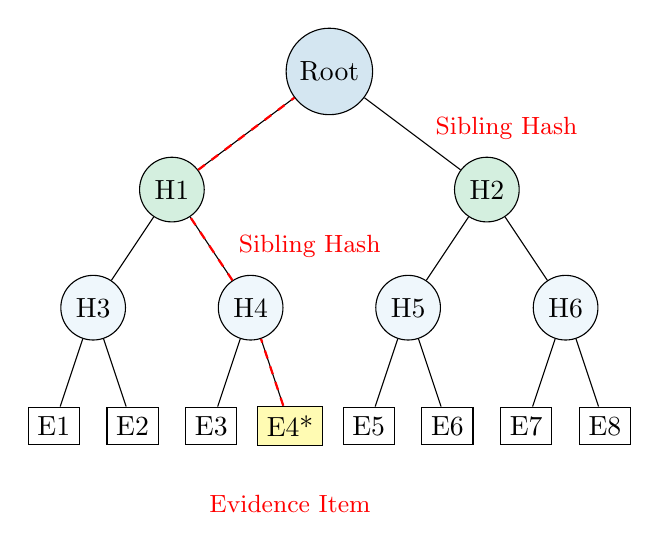
\begin{tikzpicture}[
    level distance=1.5cm,
    level 1/.style={sibling distance=4cm},
    level 2/.style={sibling distance=2cm},
    level 3/.style={sibling distance=1cm}
]

% Merkle Tree Structure
\node[circle, draw, fill=ciafblue!20] (root) {Root}
    child {
        node[circle, draw, fill=ciafgreen!20] (h1) {H1}
        child {
            node[circle, draw, fill=ciaflightblue!20] (h3) {H3}
            child {node[rectangle, draw, fill=white] (e1) {E1}}
            child {node[rectangle, draw, fill=white] (e2) {E2}}
        }
        child {
            node[circle, draw, fill=ciaflightblue!20] (h4) {H4}
            child {node[rectangle, draw, fill=white] (e3) {E3}}
            child {node[rectangle, draw, fill=yellow!30] (e4) {E4*}}
        }
    }
    child {
        node[circle, draw, fill=ciafgreen!20] (h2) {H2}
        child {
            node[circle, draw, fill=ciaflightblue!20] (h5) {H5}
            child {node[rectangle, draw, fill=white] (e5) {E5}}
            child {node[rectangle, draw, fill=white] (e6) {E6}}
        }
        child {
            node[circle, draw, fill=ciaflightblue!20] (h6) {H6}
            child {node[rectangle, draw, fill=white] (e7) {E7}}
            child {node[rectangle, draw, fill=white] (e8) {E8}}
        }
    };

% Proof path highlighting
\draw[thick, red, dashed] (e4) -- (h4);
\draw[thick, red, dashed] (h4) -- (h1);
\draw[thick, red, dashed] (h1) -- (root);

% Add proof path labels
\node[below=0.5cm of e4, text=red] {\small Evidence Item};
\node[above=0.1cm of h4, xshift=0.75cm, text=red] {\small Sibling Hash};
\node[above=0.1cm of h2, xshift=0.25cm, text=red] {\small Sibling Hash};

\end{tikzpicture}
\caption{Merkle Tree Verification Path for Evidence Item E4}
\label{fig:merkle_proof}
\end{figure}

\begin{technicalbox}
\textbf{Merkle Proof Verification Process}

To verify evidence item E4 belongs to the committed batch without downloading the entire tree, the verifier needs only a minimal \textbf{proof path} consisting of sibling hashes:

\textbf{Required Elements:}
\begin{itemize}
\item \textbf{Evidence Item:} E4 (the item being verified)
\item \textbf{Sibling Hash:} Hash(E3) - E4's direct sibling
\item \textbf{Uncle Hash:} H3 - the sibling of H4's parent 
\item \textbf{Uncle Hash:} H2 - the sibling of H1's parent
\end{itemize}

\textbf{Verification Steps:}
\begin{enumerate}
\item \textbf{Compute H4:} Hash(E3 || E4) using E4 and its sibling Hash(E3)
\item \textbf{Compute H1:} Hash(H3 || H4) using computed H4 and provided H3
\item \textbf{Compute Root:} Hash(H1 || H2) using computed H1 and provided H2
\item \textbf{Verify:} Compare computed root with the trusted root hash
\end{enumerate}

\textbf{Security Property:} If E4 was tampered with, the computed root would differ from the trusted root, proving the evidence was modified. This provides cryptographic proof of integrity with logarithmic verification complexity.
\end{technicalbox}

\subsection{Audit Trail Flowchart}

\begin{figure}[H]
\centering
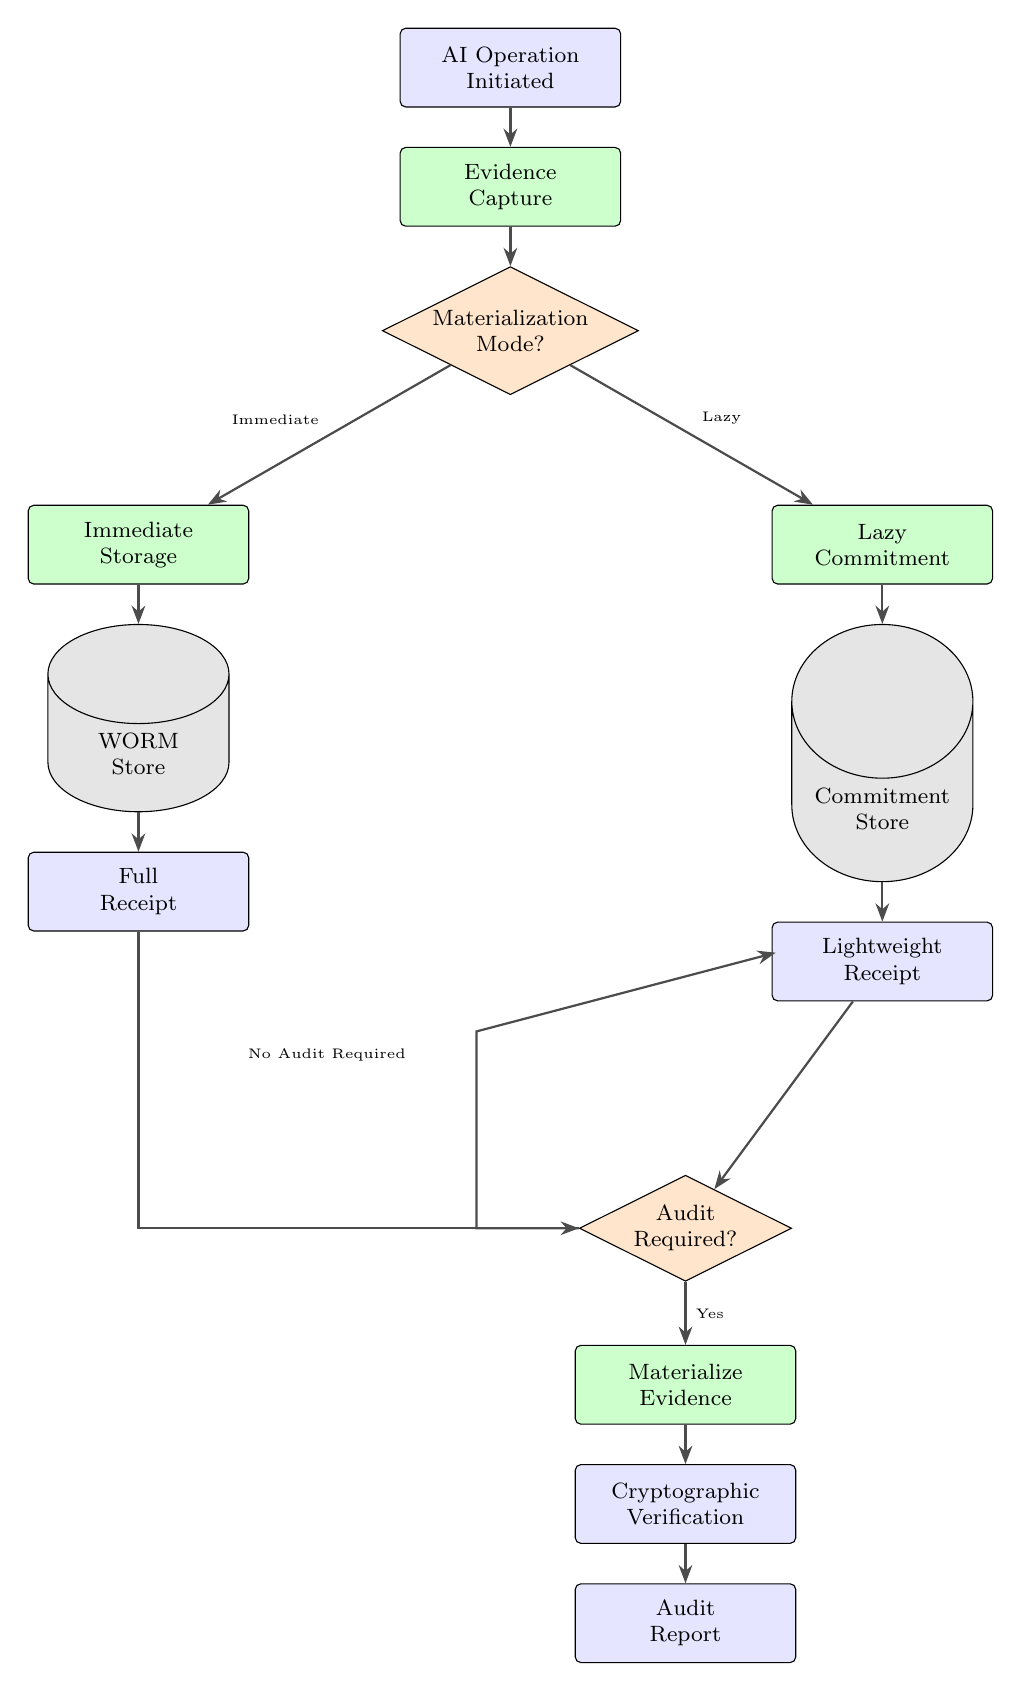
\begin{tikzpicture}[
    node distance=1.2cm,
    >=Stealth,
    box/.style={
        rectangle, draw, fill=blue!10,
        minimum width=2.8cm, minimum height=1.0cm,
        rounded corners=2pt, font=\footnotesize, align=center
    },
    decision/.style={
        diamond, draw, fill=orange!20,
        aspect=2, inner sep=1pt, minimum width=2.5cm,
        font=\footnotesize, align=center
    },
    process/.style={
        rectangle, draw, fill=green!20,
        minimum width=2.8cm, minimum height=1.0cm,
        rounded corners=2pt, font=\footnotesize, align=center
    },
    storage/.style={
        shape=cylinder, shape border rotate=90,
        draw, fill=gray!20,
        minimum width=2.3cm, minimum height=1.2cm,
        font=\footnotesize, align=center
    },
    arrow/.style={->, line width=0.8pt, draw=black!70}
]

% Flow nodes - Main path with reduced spacing
\node[box] (start) {AI Operation\\Initiated};
\node[process, below=.5cm of start] (capture) {Evidence\\Capture};
\node[decision, below=.5cm of capture] (mode) {Materialization\\Mode?};

% Branching paths with reduced spacing
\node[process, below left=1.8cm and 2.5cm of mode] (immediate) {Immediate\\Storage};
\node[process, below right=1.8cm and 2.5cm of mode] (lazy) {Lazy\\Commitment};

% Storage nodes
\node[storage, below=.5cm of immediate] (store1) {WORM\\Store};
\node[storage, below=.5cm of lazy] (store2) {Commitment\\Store};

% Receipt nodes
\node[box, below=.5cm of store1] (receipt1) {Full\\Receipt};
\node[box, below=.5cm of store2] (receipt2) {Lightweight\\Receipt};

% Audit decision and process - reduced spacing
\node[decision, below=2.2cm of receipt2, xshift=-2.5cm] (audit) {Audit\\Required?};
\node[process, below=.8cm of audit] (materialize) {Materialize\\Evidence};
\node[box, below=.5cm of materialize] (verify) {Cryptographic\\Verification};
\node[box, below=.5cm of verify] (report) {Audit\\Report};

% Flow arrows
\draw[arrow] (start) -- (capture);
\draw[arrow] (capture) -- (mode);
\draw[arrow] (mode) -- node[midway, above left, font=\tiny] {Immediate} (immediate);
\draw[arrow] (mode) -- node[midway, above right, font=\tiny] {Lazy} (lazy);
\draw[arrow] (immediate) -- (store1);
\draw[arrow] (lazy) -- (store2);
\draw[arrow] (store1) -- (receipt1);
\draw[arrow] (store2) -- (receipt2);

% Connection to audit decision
\draw[arrow] (receipt1) |- (audit);
\draw[arrow] (receipt2) -- (audit);

% Audit flow (Yes)
\draw[arrow] (audit) -- node[midway, right, font=\tiny] {Yes} (materialize);
\draw[arrow] (materialize) -- (verify);
\draw[arrow] (verify) -- (report);

% No-audit path (bypass) - simplified
\coordinate (exit1) at ($(audit.west)+(-1.3cm,0)$);
\coordinate (exit2) at ($(audit.west)+(-1.3cm,2.5cm)$);
\coordinate (exit3) at ($(audit.west)+(2.5cm,3.5cm)$);
\draw[arrow] (audit.west) -- (exit1) -- (exit2) -- (exit3);
\node[above, font=\tiny] at ($(exit2)!-0.5!(exit3)$) {No Audit Required};

\end{tikzpicture}
\caption{CIAF Audit Trail Processing Flow. Default deployment assumes co-location with the model; API exposure is optional and not required by this flow.}
\label{fig:audit_flow}
\end{figure}

\begin{technicalbox}
\textbf{Audit Trail Flowchart Explanation}

The flowchart illustrates CIAF's dual-mode evidence processing architecture, optimizing for both real-time performance and comprehensive auditability:

\textbf{Evidence Capture Phase:}
\begin{itemize}
\item \textbf{AI Operation Initiated:} Any AI system operation (training, inference, evaluation) triggers evidence capture
\item \textbf{Evidence Capture:} Critical audit data (inputs, outputs, model state, compliance metrics) recorded with timestamps
\end{itemize}

\textbf{Materialization Decision:}
\begin{itemize}
\item \textbf{Immediate Mode:} High-risk operations store complete evidence immediately to WORM storage
\item \textbf{Lazy Mode:} Routine operations generate lightweight receipts (1-2KB) with cryptographic commitments
\end{itemize}

\textbf{Storage Strategy:}
\begin{itemize}
\item \textbf{WORM Store:} Immutable storage for complete audit evidence with full regulatory compliance
\item \textbf{Commitment Store:} Efficient storage of cryptographic receipts enabling on-demand materialization
\end{itemize}

\textbf{Audit Activation:}
\begin{itemize}
\item \textbf{No Audit Required:} Lightweight receipts remain stored with minimal overhead
\item \textbf{Audit Required:} Triggers materialization process reconstructing complete evidence from receipts
\item \textbf{Cryptographic Verification:} SHA-256 hash chains and Ed25519 signatures validate evidence integrity
\item \textbf{Audit Report:} Generates comprehensive regulatory compliance documentation
\end{itemize}

\textbf{Key Advantages:}
\begin{itemize}
\item \textbf{85\% Storage Reduction:} Lazy materialization minimizes storage costs during normal operations
\item \textbf{Regulatory Compliance:} Both modes generate audit evidence meeting strict regulatory requirements
\item \textbf{Performance Optimization:} Minimal latency impact on AI system operations
\item \textbf{Cryptographic Integrity:} Tamper-evident audit trails with mathematical proof of integrity
\end{itemize}
\end{technicalbox}

\subsection{References}

\begin{enumerate}
\item European Commission. \textit{Regulation (EU) 2024/1689 of the European Parliament and of the Council laying down harmonised rules on artificial intelligence (Artificial Intelligence Act)}. Official Journal of the European Union, 2024.

\item National Institute of Standards and Technology. \textit{AI Risk Management Framework (AI RMF 1.0)}. NIST AI 100-1, January 2023.

\item Bray, T. \textit{The JavaScript Object Notation (JSON) Data Interchange Format}. RFC 8259, December 2017.

\item Gibson, J., Eveleigh, M., Gómez-Miralles, L., et al. \textit{JSON Canonicalization Scheme (JCS)}. RFC 8785, June 2020.

\item National Institute of Standards and Technology. \textit{Secure Hash Standard (SHS)}. FIPS PUB 180-4, August 2015.

\item Josefsson, S. and Liusvaara, I. \textit{Edwards-Curve Digital Signature Algorithm (EdDSA)}. RFC 8032, January 2017.

\item Nakamoto, S. \textit{Bitcoin: A Peer-to-Peer Electronic Cash System}. 2008.

\item Office of Management and Budget. \textit{Memorandum for the Heads of Executive Departments and Agencies: Advancing Governance, Innovation, and Risk Management for Agency Use of Artificial Intelligence}. M-24-10, March 2024.

\item European Medicines Agency. \textit{Guideline on Software as Medical Device (SaMD): Clinical Evaluation}. EMA/CHMP/SWP/367094/2018, 2021.

\item Federal Financial Institutions Examination Council. \textit{Model Risk Management Guidance}. Supervisory Guidance SR 11-7, 2011.
\end{enumerate}

\section{Glossary}

\begin{technicalbox}
\textbf{Key Terms \& Concepts}
\begin{itemize}
\item \textbf{CIAF:} Cognitive Insight Audit Framework - cryptographically verifiable AI governance architecture
\item \textbf{LCM:} Lazy Capsule Materialization - deferred evidence reconstruction with 85\% storage reduction
\item \textbf{WORM:} Write-Once-Read-Many - immutable storage semantics preventing evidence modification
\item \textbf{XAI:} Explainable AI - interpretability methods (SHAP, LIME) with regulatory compliance mapping
\item \textbf{RFC 8785:} Canonical JSON standard ensuring cross-platform hash consistency
\item \textbf{Receipt:} Lightweight cryptographic commitment (1-2KB) enabling deferred audit trail materialization
\item \textbf{Capsule:} Full audit evidence container materialized on-demand from lightweight receipts
\item \textbf{Gate:} Policy-driven compliance checkpoint returning PASS/WARN/FAIL/REVIEW status with signed receipts
\end{itemize}
\end{technicalbox}

\section{Regulatory Framework Coverage}

This document addresses compliance requirements across multiple regulatory frameworks. The following section provides direct links to the regulations, specific articles covered, and CIAF's implementation approach for each framework.

\subsection{European Union Regulations}

\subsubsection{EU AI Act (Regulation 2024/1689)}
\begin{valuebox}
\textbf{Official Title:} Regulation (EU) 2024/1689 laying down harmonised rules on artificial intelligence\\
\textbf{Official Link:} \href{https://eur-lex.europa.eu/eli/reg/2024/1689/oj}{\textcolor{blue}{EUR-Lex Official Publication}}\\
\textbf{Effective Date:} August 1, 2024 (Full enforcement: August 2026)

\textbf{Key Articles Addressed by CIAF:}
\begin{itemize}
\item \textbf{Article 11} - Obligations for high-risk AI systems: CIAF lightweight receipts provide required documentation
\item \textbf{Article 12} - Quality management systems: Evidence strength classification supports systematic quality control
\item \textbf{Article 13} - Transparency obligations: Provenance chains enable algorithmic transparency requirements
\item \textbf{Article 14} - Human oversight requirements: CIAF HITL gates enforce human-in-the-loop compliance
\item \textbf{Article 15} - Accuracy and robustness: Cryptographic commitments ensure model performance verification
\end{itemize}

\textbf{CIAF Implementation:} Automated compliance mapping, real-time bias detection, human oversight gates, and cryptographic audit trails meeting EU AI Act requirements for high-risk AI systems.
\end{valuebox}

\subsubsection{General Data Protection Regulation (GDPR)}
\begin{technicalbox}
\textbf{Official Title:} Regulation (EU) 2016/679 on the protection of natural persons\\
\textbf{Official Link:} \href{https://eur-lex.europa.eu/eli/reg/2016/679/oj}{\textcolor{blue}{EUR-Lex GDPR Text}}\\
\textbf{Effective Date:} May 25, 2018

\textbf{Key Articles Addressed by CIAF:}
\begin{itemize}
\item \textbf{Article 22} - Automated decision-making: XAI integration provides right to explanation
\item \textbf{Article 25} - Data protection by design: Privacy-preserving audit architecture
\item \textbf{Article 30} - Records of processing: Comprehensive audit trail generation
\item \textbf{Article 35} - Data protection impact assessment: Automated DPIA documentation
\end{itemize}

\textbf{CIAF Implementation:} Privacy-preserving evidence capture, explainable AI compliance, automated DPIA generation, and audit trail protection meeting GDPR transparency requirements.
\end{technicalbox}

\subsection{United States Regulations}

\subsubsection{NIST AI Risk Management Framework}
\begin{valuebox}
\textbf{Official Title:} NIST AI Risk Management Framework (AI RMF 1.0)\\
\textbf{Official Link:} \href{https://www.nist.gov/itl/ai-risk-management-framework}{\textcolor{blue}{NIST AI RMF Official Page}}\\
\textbf{Publication Date:} January 26, 2023

\textbf{Key Functions Addressed by CIAF:}
\begin{itemize}
\item \textbf{GOVERN-1.1} - AI governance policies: Policy-driven gate configuration
\item \textbf{MAP-2.3} - Risk measurement and assessment: Evidence strength classification
\item \textbf{MEASURE-2.1} - Test and validation: Cryptographic verification of model performance
\item \textbf{MEASURE-4.1} - Harmful bias monitoring: Automated bias detection gates
\item \textbf{GOVERN-2.1} - Oversight processes: Human-in-the-loop compliance architecture
\end{itemize}

\textbf{CIAF Implementation:} Risk-based compliance gates, continuous bias monitoring, stakeholder impact assessment, and comprehensive AI lifecycle governance aligned with NIST RMF categories.
\end{valuebox}

\subsubsection{OMB Memorandum M-24-10}
\begin{technicalbox}
\textbf{Official Title:} Advancing Governance, Innovation, and Risk Management for Agency Use of AI\\
\textbf{Official Link:} \href{https://www.whitehouse.gov/wp-content/uploads/2024/03/M-24-10-Advancing-Governance-Innovation-and-Risk-Management-for-Agency-Use-of-Artificial-Intelligence.pdf}{\textcolor{blue}{White House OMB M-24-10}}\\
\textbf{Effective Date:} March 28, 2024

\textbf{Key Requirements Addressed by CIAF:}
\begin{itemize}
\item \textbf{Section 3} - Minimum practices for AI governance: Comprehensive audit trail generation
\item \textbf{Section 4} - Safety and security requirements: Cryptographic evidence integrity
\item \textbf{Section 5} - Transparency and accountability: Public algorithm registry capabilities
\item \textbf{Section 6} - Continuous monitoring: Real-time performance and bias monitoring
\end{itemize}

\textbf{CIAF Implementation:} Government-compliant algorithmic transparency, public audit verification, continuous AI system monitoring, and appeals process documentation for contested decisions.
\end{technicalbox}

\subsection{Industry-Specific Regulations}

\subsubsection{Healthcare: FDA Software as Medical Device (SaMD)}
\begin{valuebox}
\textbf{Official Title:} Software as Medical Device (SaMD): Clinical Evaluation Guidance\\
\textbf{Official Link:} \href{https://www.fda.gov/medical-devices/digital-health-center-excellence/software-medical-device-samd}{\textcolor{blue}{FDA SaMD Guidance}}\\
\textbf{Updates:} Ongoing (AI/ML guidance updated 2021-2024)

\textbf{Key Requirements Addressed by CIAF:}
\begin{itemize}
\item \textbf{Clinical Validation:} Cryptographic evidence of AI model performance on clinical data
\item \textbf{Risk Classification:} Automated IEC 62304 risk assessment and documentation
\item \textbf{Change Control:} Immutable audit trail of model updates and revalidation
\item \textbf{Post-Market Surveillance:} Real-world performance monitoring with regulatory reporting
\end{itemize}

\textbf{CIAF Implementation:} Medical device compliance automation, clinical validation evidence capture, FDA 510(k) documentation support, and post-market surveillance integration.
\end{valuebox}

\subsubsection{Financial Services: Fair Credit Reporting Act (FCRA)}
\begin{technicalbox}
\textbf{Official Title:} Fair Credit Reporting Act (15 U.S.C. §1681)\\
\textbf{Official Link:} \href{https://www.ftc.gov/legal-library/browse/statutes/fair-credit-reporting-act}{\textcolor{blue}{FTC FCRA Information}}\\
\textbf{AI Guidance:} Updated with algorithmic decision-making requirements

\textbf{Key Requirements Addressed by CIAF:}
\begin{itemize}
\item \textbf{Section 615} - Adverse action notices: Automated explanation generation for AI decisions
\item \textbf{Section 604} - Permissible purposes: Purpose-binding evidence in audit trails
\item \textbf{Section 611} - Dispute procedures: Auditable review process for contested AI decisions
\item \textbf{Section 605} - Accuracy requirements: Model performance verification and bias monitoring
\end{itemize}

\textbf{CIAF Implementation:} Fair lending transparency, automated adverse action documentation, algorithmic bias detection, and dispute resolution audit trails for financial AI systems.
\end{technicalbox}

\subsubsection{International Standards}

\begin{valuebox}
\textbf{ISO/IEC 23053:2022} - Framework for AI risk management\\
\textbf{Link:} \href{https://www.iso.org/standard/74438.html}{\textcolor{blue}{ISO 23053 Standard}}\\
\textbf{Coverage:} Risk assessment methodologies, governance structures, continuous monitoring

\textbf{ISO/IEC 23894:2023} - AI risk management process\\
\textbf{Link:} \href{https://www.iso.org/standard/77304.html}{\textcolor{blue}{ISO 23894 Standard}}\\
\textbf{Coverage:} Systematic risk management, stakeholder engagement, documentation requirements

\textbf{ISO/IEC 42001:2023} - AI management systems\\
\textbf{Link:} \href{https://www.iso.org/standard/81230.html}{\textcolor{blue}{ISO 42001 Standard}}\\
\textbf{Coverage:} Management system requirements, organizational governance, continual improvement
\end{valuebox}

\subsection{Emerging Regulatory Developments}

\begin{infobox}
\textbf{Regulatory Tracking:} CIAF continuously monitors emerging regulations including:
\begin{itemize}
\item \textbf{California SB-1001:} Bot disclosure requirements for AI systems
\item \textbf{UK AI White Paper:} Principles-based regulatory approach for AI governance
\item \textbf{Singapore Model AI Governance:} Voluntary AI governance framework and implementation guidance
\item \textbf{China AI Regulation:} Draft measures for algorithmic recommendation and deep synthesis
\item \textbf{Canada AIDA:} Proposed Artificial Intelligence and Data Act requirements
\end{itemize}

The CIAF framework is designed to adapt to evolving regulatory requirements through its modular compliance architecture and policy-driven configuration system.
\end{infobox}

\vfill

\begin{center}
\textcolor{ciafgray}{\rule{0.8\textwidth}{0.4pt}}\\
\vspace{0.3cm}
\textbf{AI Assistance Disclosure}\\
\vspace{0.2cm}
This research work utilized artificial intelligence tools as assistants in the development process. AI assistance was employed for code creation, documentation drafting, and technical writing support. The author maintained oversight throughout the entire process and takes full responsibility for the final code, documentation, and research content. All AI-generated content was reviewed, edited, and validated by the author to ensure accuracy, originality, and alignment with research objectives.\\
\vspace{0.3cm}
\textcolor{ciafgray}{\rule{0.8\textwidth}{0.4pt}}\\
\vspace{0.3cm}
\textbf{License \& Citation}\\
\vspace{0.3cm}
© 2025 Denzil James Greenwood. All rights reserved.\\
\textbf{Software:} Licensed under Apache 2.0 • \textbf{Documentation:} Licensed under CC BY 4.0\\
\textbf{Trademarks:} Cognitive Insight™ and LCM™ are unregistered trademarks used in connection with ongoing research on verifiable AI governance and auditability.\\
\vspace{0.2cm}
\textbf{Suggested Citation:}\\
\textit{Greenwood, D.J. (2025). CIAF + LCM Research Disclosure Portfolio: Cognitive Insight Audit Framework with Lazy Capsule Materialization. Independent Research Publication. Available at: https://github.com/DenzilGreenwood/CIAF\_Model\_Creation}\\
\vspace{0.25cm}
\textbf{Academic Citation (BibTeX):}\\
\begin{verbatim}
@techreport{greenwood2025ciaf,
  title={CIAF + LCM Research Disclosure Portfolio: Cognitive Insight Audit 
  Framework with Lazy Capsule Materialization},
  author={Greenwood, Denzil James},
  year={2025},
  institution={Independent Research},
  type={Technical Report},
  url={https://github.com/DenzilGreenwood/CIAF_Model_Creation},
  note={Apache 2.0 Licensed}
}
\end{verbatim}
\vspace{0.25cm}
\textcolor{ciafgray}{\rule{0.8\textwidth}{0.4pt}}\\
\vspace{0.4cm}
\textbf{Contact Information}\\
\vspace{0.25cm}
Denzil James Greenwood | Independent Researcher\\
Email: Founder@cognitiveinsight.ai\\
LinkedIn: www.linkedin.com/in/denzil-james-greenwood\\
Website: CognitiveInsight.ai\\
Repository: github.com/DenzilGreenwood/CIAF\_Model\_Creation\\
\vspace{0.25cm}
\textit{Open to collaboration, peer review, and funded research opportunities}\\
\vspace{0.4cm}
\textcolor{ciafgray}{\rule{0.8\textwidth}{0.25pt}}
\end{center}

\end{document}
